\chapter{Navigation Policy Evaluation Studies}
\label{chap:7_navigation_policy_evaluation_studies}

In this chapter, we present and evaluate our approach in developing an efficient collision-free navigation policy. Our approach is presented in the context of the curriculum, where we share the step-by-step decisions and thought process for training our policy.
The final policy is then evaluated, where we assess its performance in its training environment and its ability to generalise to new environments.

For our thesis, training and simulation was done on an Intel(R) Core(TM) i9-10940X CPU @ 3.30GHz desktop PC, with a NVIDIA GeForce RTX 3090 GPU. 

\section{Policy Performance along the Learning Curriculum}
\label{sec:7_learning_curriculum}
In this section, we analyse the training characteristics of our navigation policy in progressively difficult environments. In total, our curriculum is composed of 7 levels, with an initial pretraining stage. An overview of the training time and environment setup is shown in Figures \ref{tab:7_curriculum} and
\ref{tab:7_curriculum_space} respectively.
\begin{table}[hbt]
    \centering
    \begin{tabular}{||c|c|c|c||}
    \hline
    Level & No. of Obstacles & Iterations & Time \\
    \hline\hline
    0 & 0 - Pretraining & 97 & 12m \\ \hline
    1 & 0 & 95 & 11m \\ \hline
    2 & 1 & 808 & 1h 40m \\ \hline
    3 & 3 & 652 & 1h 22m \\ \hline
    4 & 5 & 1498 & 3h 12m \\ \hline
    5 & 9 & 3500 & 7h 38m \\ \hline
    \end{tabular}
    \caption{The learning curriculum for the navigation policy. The total time for training is all seven policies is 14h 15m, with 6650 total iterations. One iteration is given by the length of the trajectory $\boldsymbol{T}$, defined as 8 simulation timesteps.}
    \label{tab:7_curriculum}
\end{table}
\begin{table}[hbt]
    \centering
    \begin{tabular}{||c|c|c|c|c||}
    \hline
    Level & No. of obstacles & Env. Size & Obst. Area & Space per obst. \\  & & & & (m$^2$ / obst.) \\\hline\hline
    0 \& 1 & 0 & 16, 8 & - & - \\\hline
    2 & 1 & 16, 8 & 32 & 32.0 \\\hline
    3 & 3 & 20, 10 & 80 & 26.67 \\\hline
    4 & 5 & 20, 10 & 80 & 16.0 \\\hline
    5 & 9 & 20, 10 & 80 & 8.89 \\\hline
    \end{tabular}
    \caption{Environments used in the curriculum. We specify the ``openness'' per environment as a more intuitive measure for clutter rather than obstacle density. The obstacle area begins 6m from each end of the enclosure to allow space for the quadrotor and goal. Thus, the obstacle area is given by $A = (X - 12) \cdot Y$.}
    \label{tab:7_curriculum_space}
\end{table}
For each environment, the policy performance will be briefly analysed in the context of \textit{average return} across all environments and the \textit{episode end information} for the last 1000 episode ends.

\subsubsection{Understanding the Average Return and End Info Plots}
The average return in this case is given by the average accumulated rewards across all environments, giving an indication of the overall navigational efficiency of the robot as the reward function is centered around the quadrotor reaching its goal. 
However, to ensure that robots are constantly exploring the environment dynamics and learning collision avoidance, we specify an end episode timestep $T$ that resets the environment and places the quadrotor back to its initial position. This significantly changes the average rewards in the scenario that multiple environments are reset, producing sharp drops or spikes in the average return plots.

Since the reward is centered around reaching goal, there is a good chance that the learned policy is not exactly ideal in terms of collision avoidance. Thus, we include the the episode end label as an abstract continuous indicator of the collision rate for the current policy. We can expect that if both the collision rate and average return is high, the quadrotor is quite aggressive in flying towards goal, sacrificing some collisions in order to exploit high rewards near goal. In contrast, if both are low, we can imagine that the policy does not have an idea of how to exploit the reward system but avoids collisions, meaning it is overly conservative and does not reach the goal, despite not crashing. In the extreme case where the reward is very low and the collision rate is high, this suggests that the policy has \textit{diverged} -- i.e. the weights of the network are so far from its optimal configuration space that it is unable to perform meaningful actions. Most clearly, the desired policy is opposite of this: with maximum return and minimal collision. 
In addition, since the end information is averaged over 1000 episodes, there is a small \textit{delay} when observing the collision avoidance properties from a current policy. As a result, the policies that are collision avoidant should either have positive slopes for timeout-episodes or maintain its low collision rates for subsequent episode ends. 

Finally, we specify bounds on the quadrotor height, where the quadrotor is reset if $z$-position goes beyond $[0, 3]$. Hence, there are three ways an episode can end: through this \textit{out of bounds} in $z$, through \textit{timeout} after $T$ timesteps, or \textit{collisions} where an obstacle is $<0.2m$ away from it or there is contact on the sides.
 
\subsection{Without Obstacles}
\begin{figure}[H]
    \centering
    \begin{subfigure}[b]{\textwidth}
        \centering
        \captionsetup{justification=centering}
        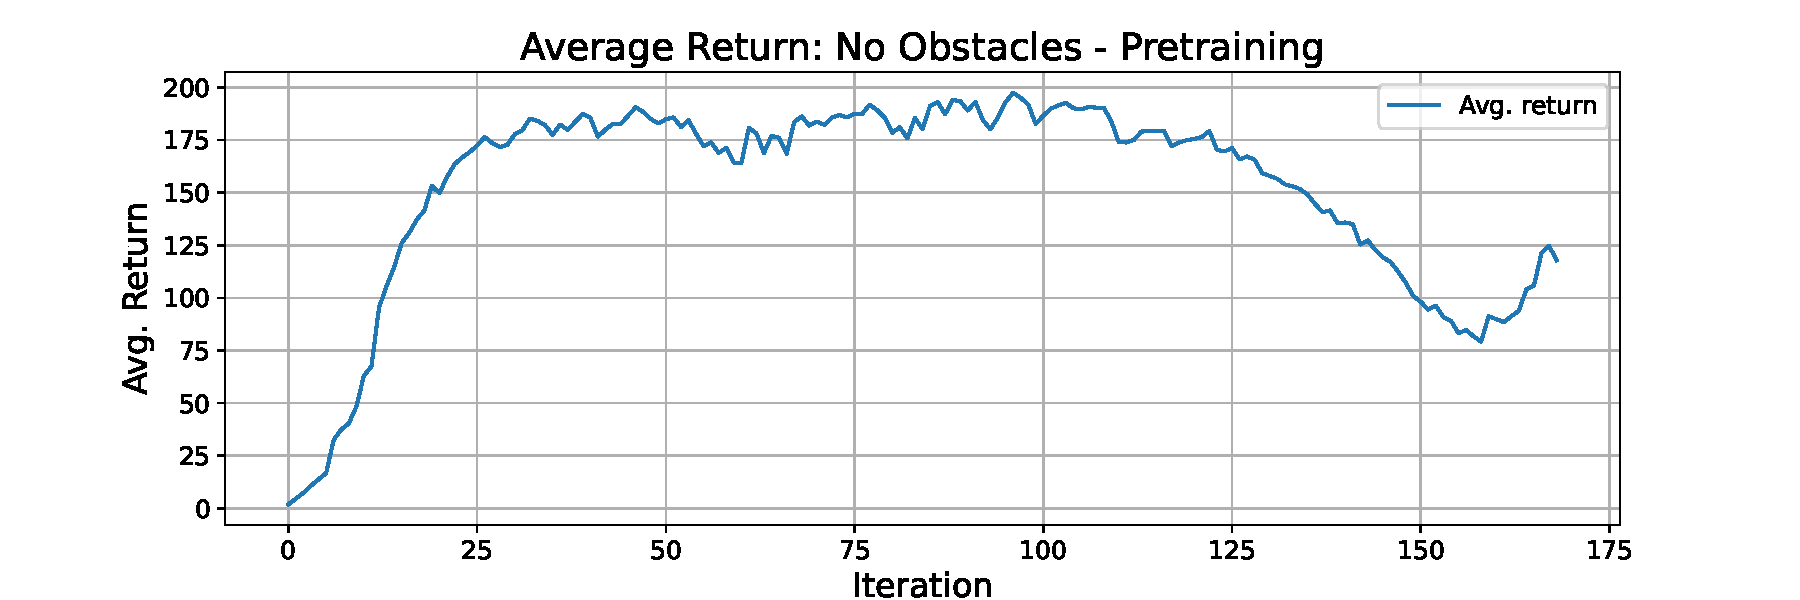
\includegraphics[width=0.99\textwidth]{figures/7_/3DCarModel_BodyObs_0_NewObs_v0_reward.pdf}
        \label{fig:0_obst_pretraining_rew}
    \end{subfigure} \\
    \begin{subfigure}[b]{\textwidth}
        \centering
        \captionsetup{justification=centering}
        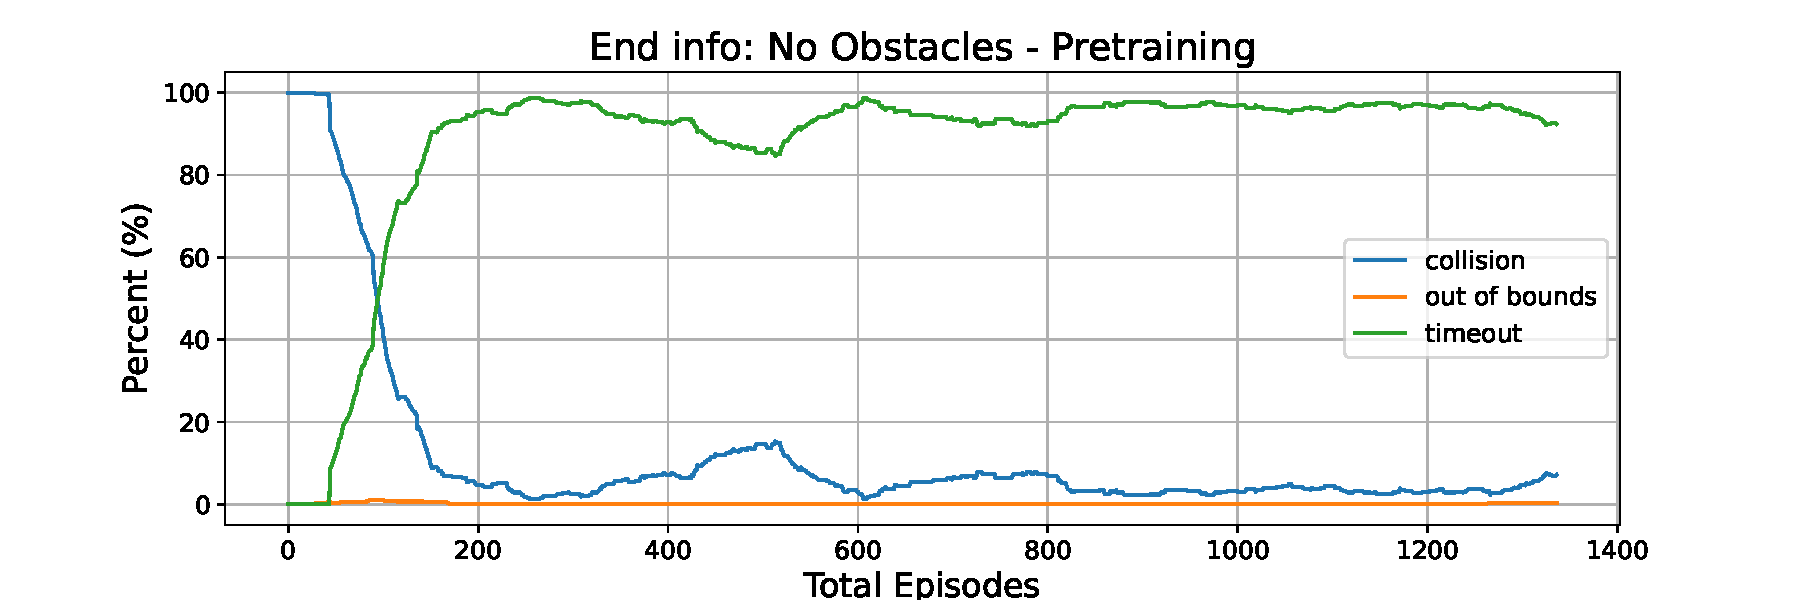
\includegraphics[width=0.99\textwidth]{figures/7_/3DCarModel_BodyObs_0_NewObs_v0_end_info.pdf}
        \label{fig:0_obst_pretraining_end}
    \end{subfigure} 
    \caption{Initialising the navigation policy. The quadrotor and goal is randomly initialised in a $[-3,3]$ area with heights $z \in [0.2, 2.0]$. The best model is selected at 97 iterations.}
    \label{fig:7_train_pretraining_no_obst}
\end{figure}
As stated in \cref{subsec:5_curriculum}, before a quadrotor learns collision avoidance, it must first learn to fly towards a goal. Given that our observation-action mapping space is quite large ($\R^{77} \rightarrow \R^{3}$), our initial guess was that navigating towards a waypoint could already be quite challenging given that we are in the continuous domain. 
With this expectation, we trained our policy with results in \cref{fig:7_train_pretraining_no_obst}.
From this figure, we can observe that pretraining is very successful, where the quadrotor steadily increases its average return at the same time its collision rate drops. By just 30 iterations (4 minutes), we see that the agent reaches its goal 100\% of the time and maximises its potential reward for most of the episode.

The next step taken is to initialise the quadrotor and goal in its new environment setup, where each are placed at the end of the environment. This is a relatively simple training stage that we expect should be completed with ease. 
\begin{figure}[htb]
    \centering
    \begin{subfigure}[b]{\textwidth}
        \centering
        \captionsetup{justification=centering}
        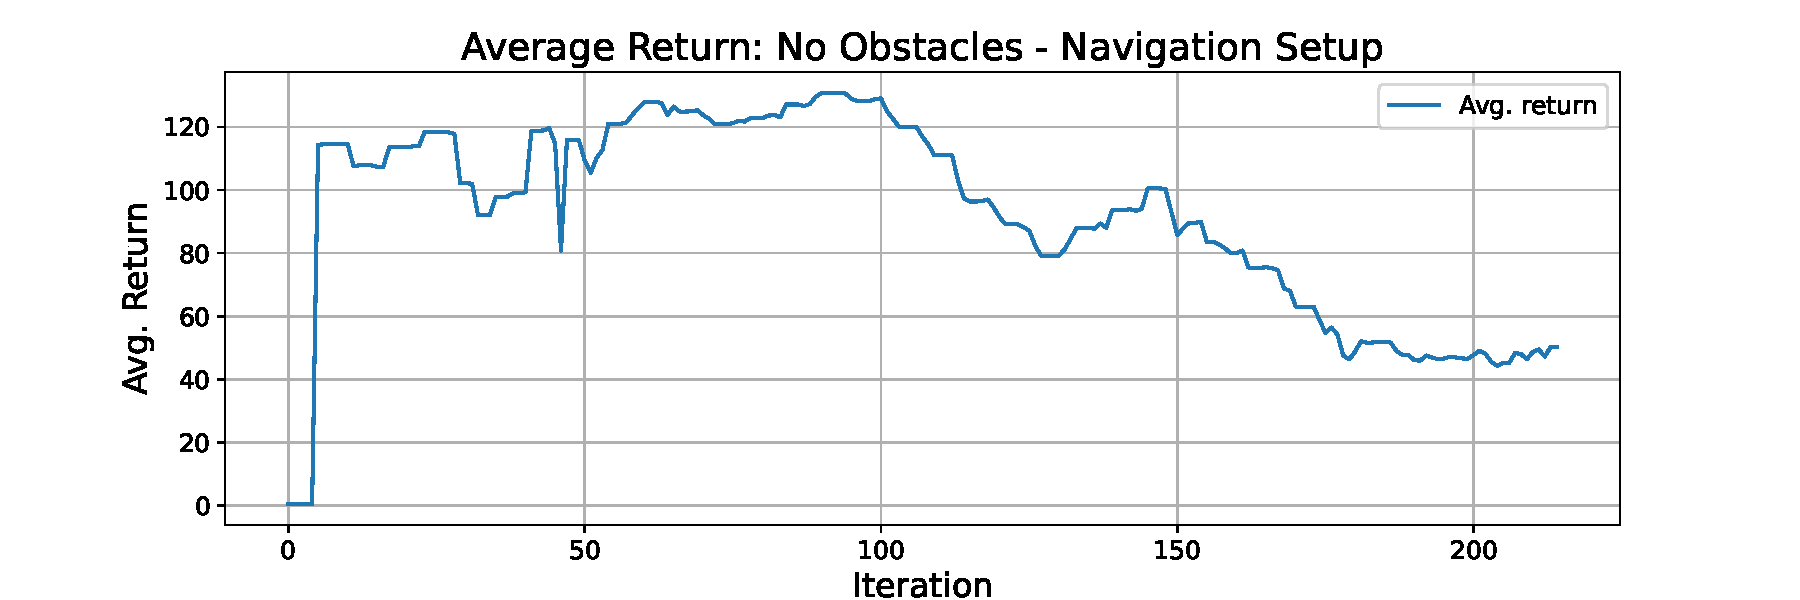
\includegraphics[width=0.99\textwidth]{figures/7_/3DCarModel_BodyObs_NavSetup_0_NewObs_v0_reward.pdf}
        \label{fig:0_obst_nav_rew}
    \end{subfigure} \\
    \begin{subfigure}[b]{\textwidth}
        \centering
        \captionsetup{justification=centering}
        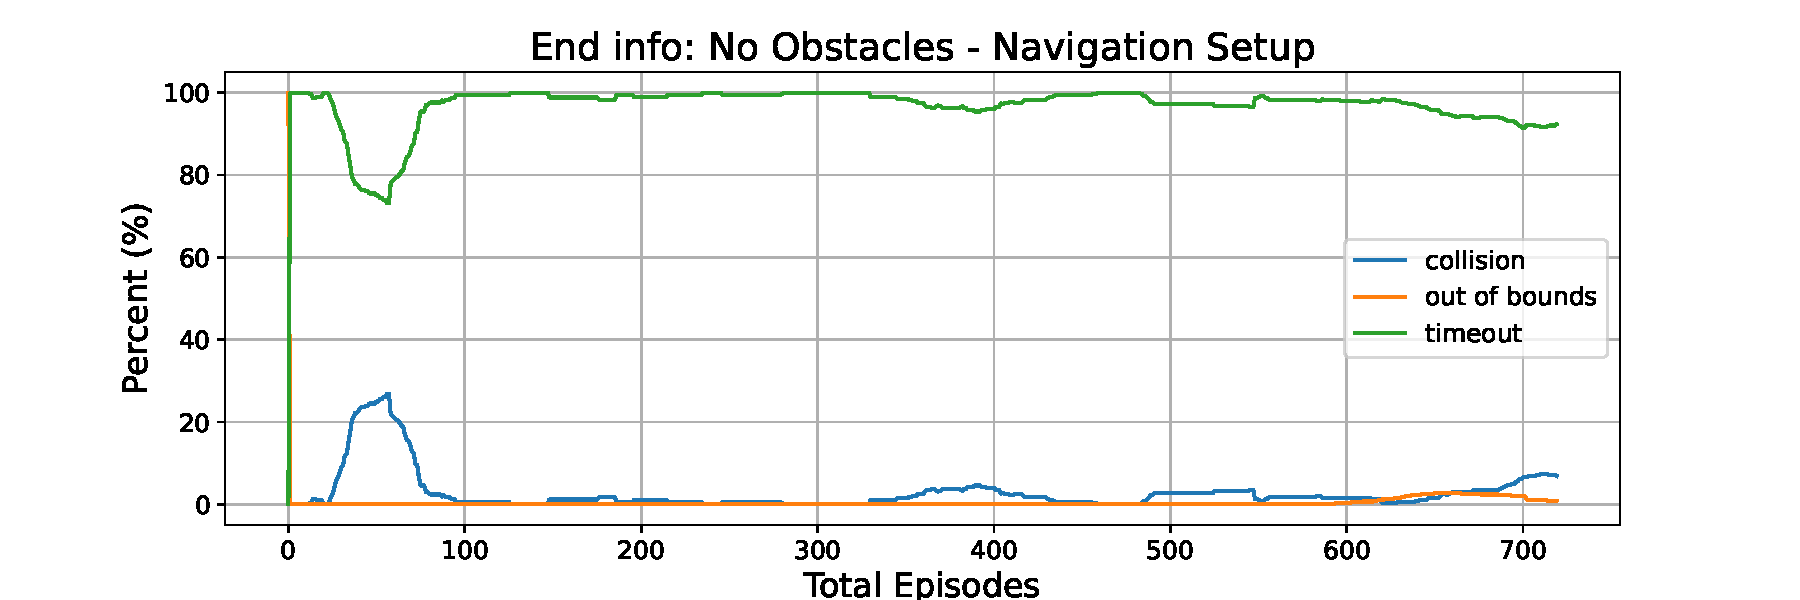
\includegraphics[width=0.99\textwidth]{figures/7_/3DCarModel_BodyObs_NavSetup_0_NewObs_v0_end_info.pdf}
        \label{fig:0_obst_nav_end}
    \end{subfigure}
    \caption{Conditioning the policy to its new state distribution. The best model is selected at 95 iterations.}
    \label{fig:7_train_nav_no_obst}
\end{figure}
From \cref{fig:7_train_nav_no_obst}, we see that this is true, where we mostly observe timeouts.

\subsection{1 Obstacle}
\label{subsec:7_1_obstacle}
Before the first obstacle is added, the agent does not necessarily have to learn to avoid close obstacles. In this situation however, obstacles are placed directly in between the quadrotor and goal, such that to achieve a low collision rate, some degree of collision avoidance is necessary.
\begin{figure}[htb]
    \centering
    \begin{subfigure}[b]{\textwidth}
        \centering
        \captionsetup{justification=centering}
        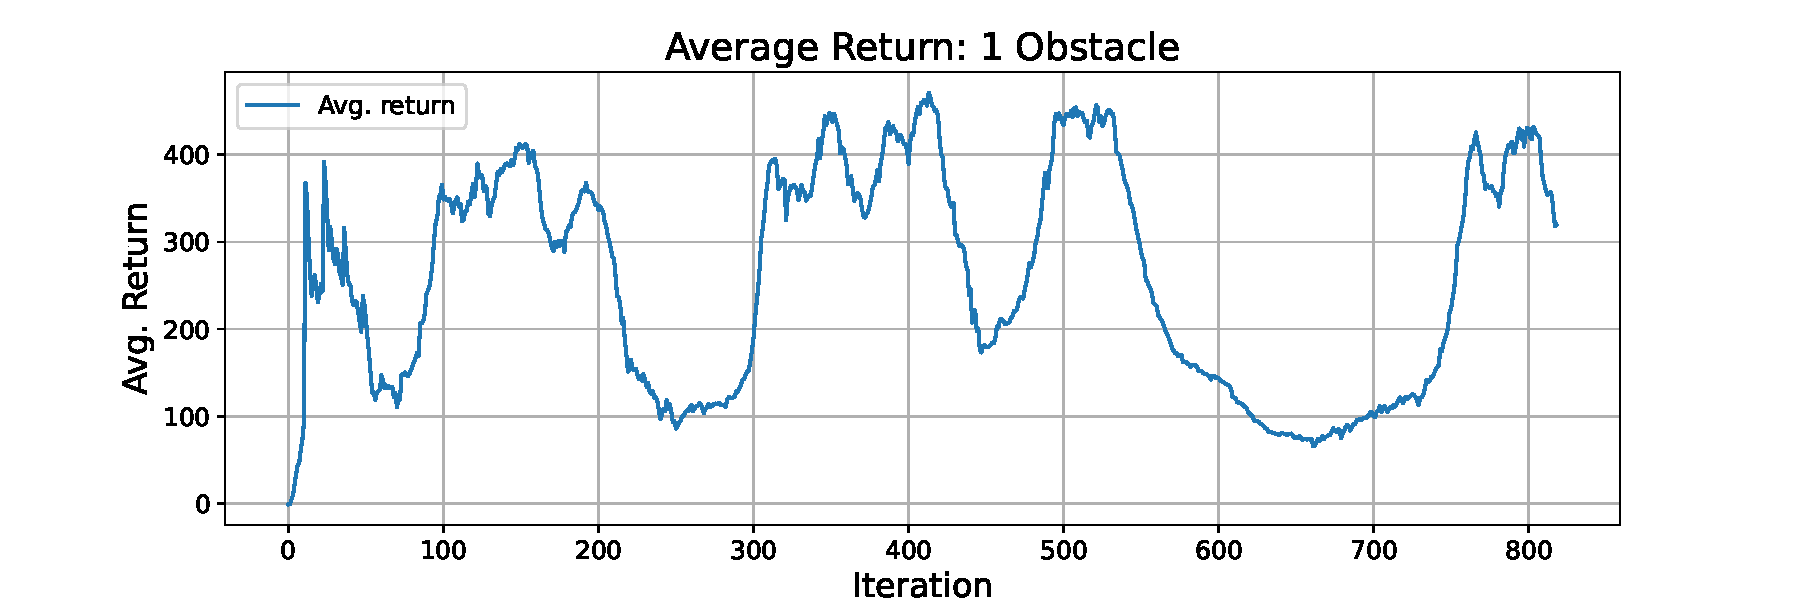
\includegraphics[width=0.99\textwidth]{figures/7_/3DCarModel_BodyObs_NavSetup_1_NewObs_v1_reward.pdf}
        \label{fig:1_obst_nav_rew}
    \end{subfigure} \\
    \begin{subfigure}[b]{\textwidth}
        \centering
        \captionsetup{justification=centering}
        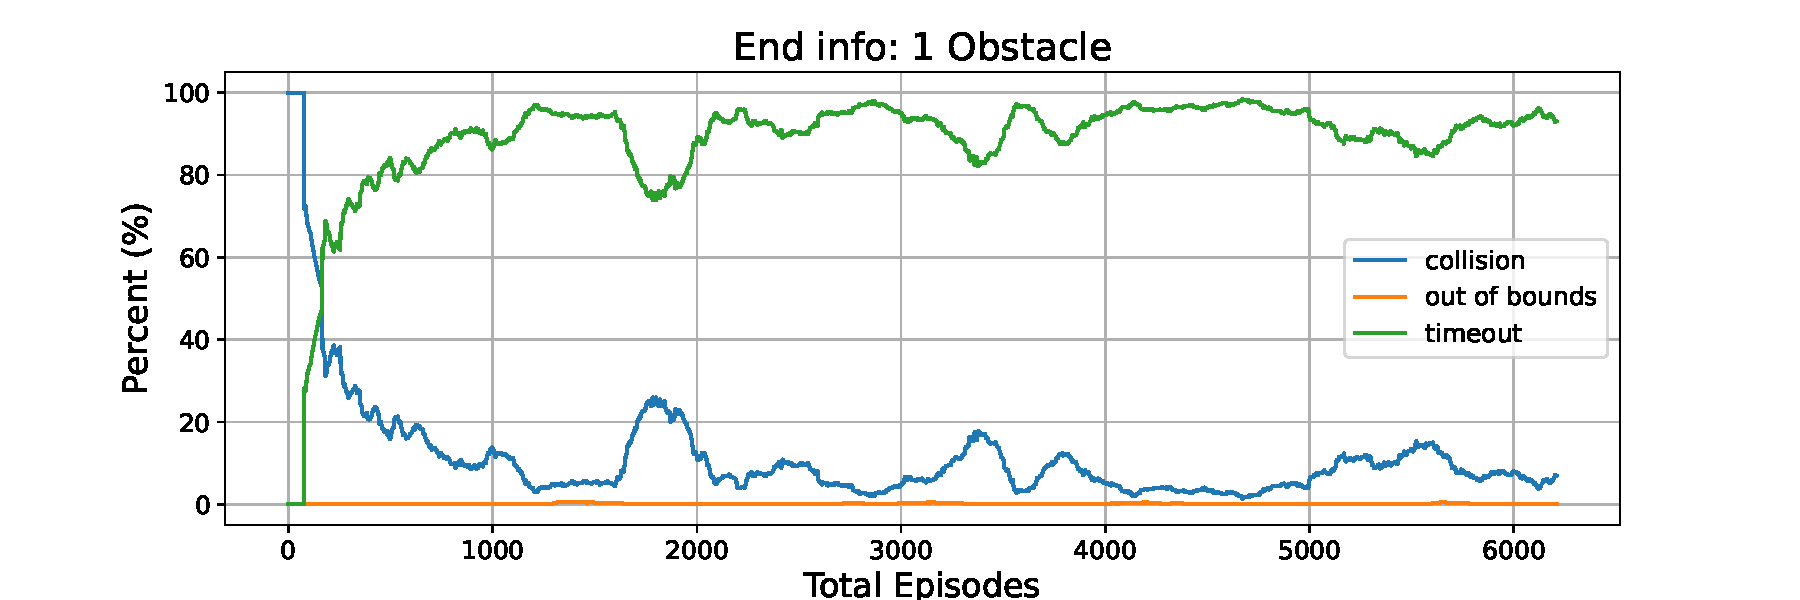
\includegraphics[width=0.99\textwidth]{figures/7_/3DCarModel_BodyObs_NavSetup_1_NewObs_v1_end_info.pdf}
        \label{fig:1_obst_nav_end}
    \end{subfigure} 
    \caption{Training with 1 obstacle. The best model is selected at 808 iterations, with an average return of 422 and timeout rate of $95.6\%$.}
    \label{fig:7_train_nav_1_obst}
\end{figure}
Despite this new challenge, we see that the quadrotor does well to cope -- steadily decreasing its collision rate to about 4\% in about 160 iterations (20 minutes), and to a minimum of about 2\% at 600 iterations. Though, in regards to policy performance, we note that the average return follows a very oscillatory behaviour which is reflected very slightly in the collision rate. Intuitively, this can be explained by the agent exploring its state-space, which consequently can be good or bad -- the quadrotor cannot know that colliding with an obstacle always leads to a negative reward until it has experienced it repeatedly from various positions. 
However, since we did surround the quadrotor in a rectangular enclosure, it was observed that the quadrotor managed to learn to not crash into walls quite early, albeit to a small degree. Just by simply stopping and turning though, is enough to pass this level.

We observe that it is not until the third oscillation in the average return that the agent finds an optimal policy which combines high total rewards with low collision rates. After this, we do observe that the collision probability falls even lower, but so too does the reward gained. Thus, we remind ourselves that we want \textit{both} navigational efficiency and conservativeness in our policy. For this training stage, we selected the model at 808, which had a good combination of both.

An early behaviour that was also observed during training is that the quadrotor learned to pick a ``favourite side'' when avoiding obstacles -- sometimes it always passed on the left, other times always on the right, despite it being more open on the other side. To try and explain this, we have to remember that neural networks are function approximators. In some sense, we can think of ``seeing the obstacle'' as a variable that is sometimes positive (or zero) in the latent code. If it is not there, we go straight, but if it is there, we turn to one side -- deterministically. We can imagine that if the agent is directly in front and in the middle of an obstacle, unless the policy is randomised to a significant extent, the same values in the input should result in the same action.

\subsection{3 Obstacles}
\label{subsec:7_3_obstacles}
Continuing onwards to three obstacles, we expect that similar to one obstacle, we should observe oscillations in the return as the agent explores different approaches to solving the navigation task. We also expect that since the obstacle has learned how to avoid one obstacle, it should be be straightforward to generalise this to three -- particularly when the objects are placed far apart.
\begin{figure}[htb]
    \centering
    \begin{subfigure}[b]{\textwidth}
        \centering
        \captionsetup{justification=centering}
        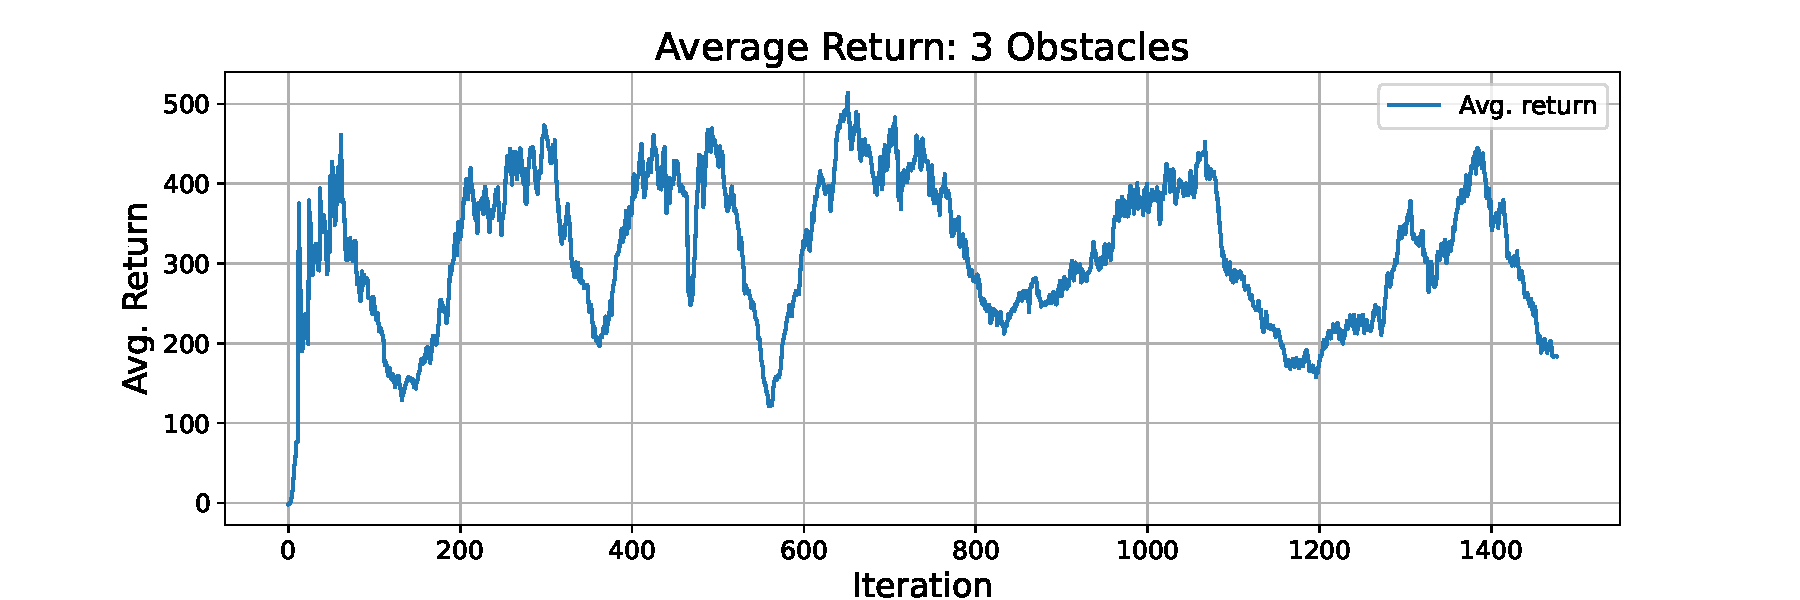
\includegraphics[width=0.99\textwidth]{figures/7_/3DCarModel_BodyObs_NavSetup_3_NewObs_v1_reward.pdf}
        \label{fig:3_obst_nav_rew}
    \end{subfigure} \\
    \begin{subfigure}[b]{\textwidth}
        \centering
        \captionsetup{justification=centering}
        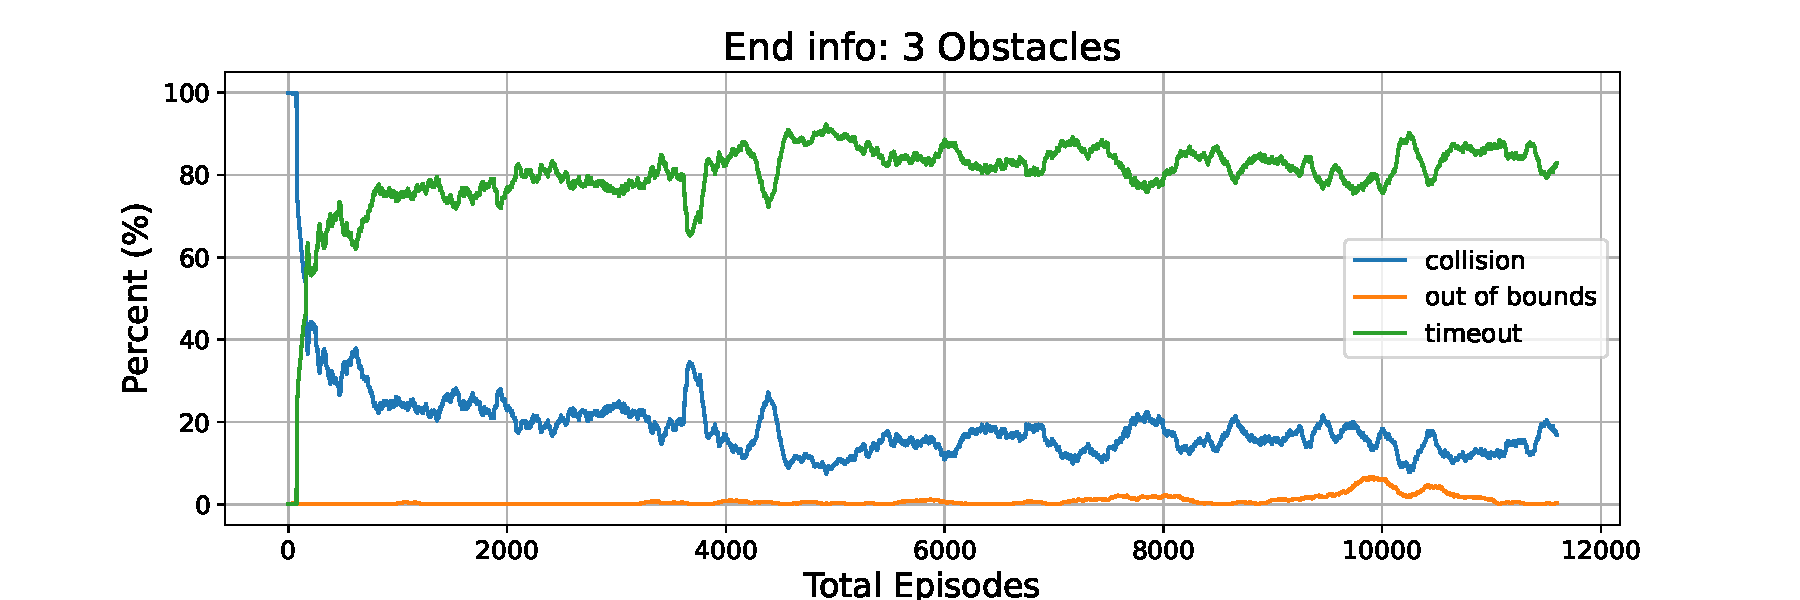
\includegraphics[width=0.99\textwidth]{figures/7_/3DCarModel_BodyObs_NavSetup_3_NewObs_v1_end_info.pdf}
        \label{fig:3_obst_nav_end}
    \end{subfigure} 
    \caption{Training with 3 obstacles. The best model is selected at 652 iterations, with an average return of 514 and timeout rate of $89.7\%$.} %1652
    \label{fig:7_train_nav_3_obst}
\end{figure}
From \cref{fig:7_train_nav_3_obst}, we see that these expectations are largely matched -- with the average accumulated reward varying significantly and the collision rates steadily increasing. From this, we observe that the a good combination of both is just about in between 600 and 700 iterations, such that we choose the best model at 652 iterations.

One of the most pertinent differences that we can observe in this scenario is that the highest timeout rates are consistently lower than before. We can accept that since the agent is essentially re-learning a more complex state-action mapping -- e.g. meeting obstacles at the edge of the environment after turning -- we do not expect high timeout rates immediately. Yet, eventually, we do expect that if it can reach the goal $>95\%$ of the time for 1-obstacle environments, it should be able to do the same here, given a similar ``optimal'' policy. 
However, this reasoning is slightly unfair since the agent now has to perform three times more collision-free manoeuvres than in the previous case. Thus, if the agent can manoeuvre past one obstacle with $95\%$ success, it is only fair to assume for a success rate of $95\%^3 \sim 85\%$ for the three obstacle environment.
From this perspective, we then see that the policy is improving, since it does achieve over an over $90\%$ timeout rate at its best point. 

\subsection{5 Obstacles}
\label{subsec:7_5_obstacles}
When approaching more cluttered environments, an effective navigation policy has to learn to carefully judge actions as a function of more than one visible obstacles. It cannot simply navigate to one side of an obstacle, but base the extent and direction of its turns from what it sees. This is a natural consideration that even takes time learn, even for humans. 
We thus expect that policy learning will progressively take longer in more complex environments as the agent learns to fine-tune this behaviour. Based on this assumption, we train the policy for significantly longer ($\approx 6800$ iterations) and increase the end episode timestep $T$ to compensate for manoeuvring time. The result of which is shown in \cref{fig:7_train_nav_5_obst}.
\begin{figure}[htb]
    \centering
    \begin{subfigure}[b]{\textwidth}
        \centering
        \captionsetup{justification=centering}
        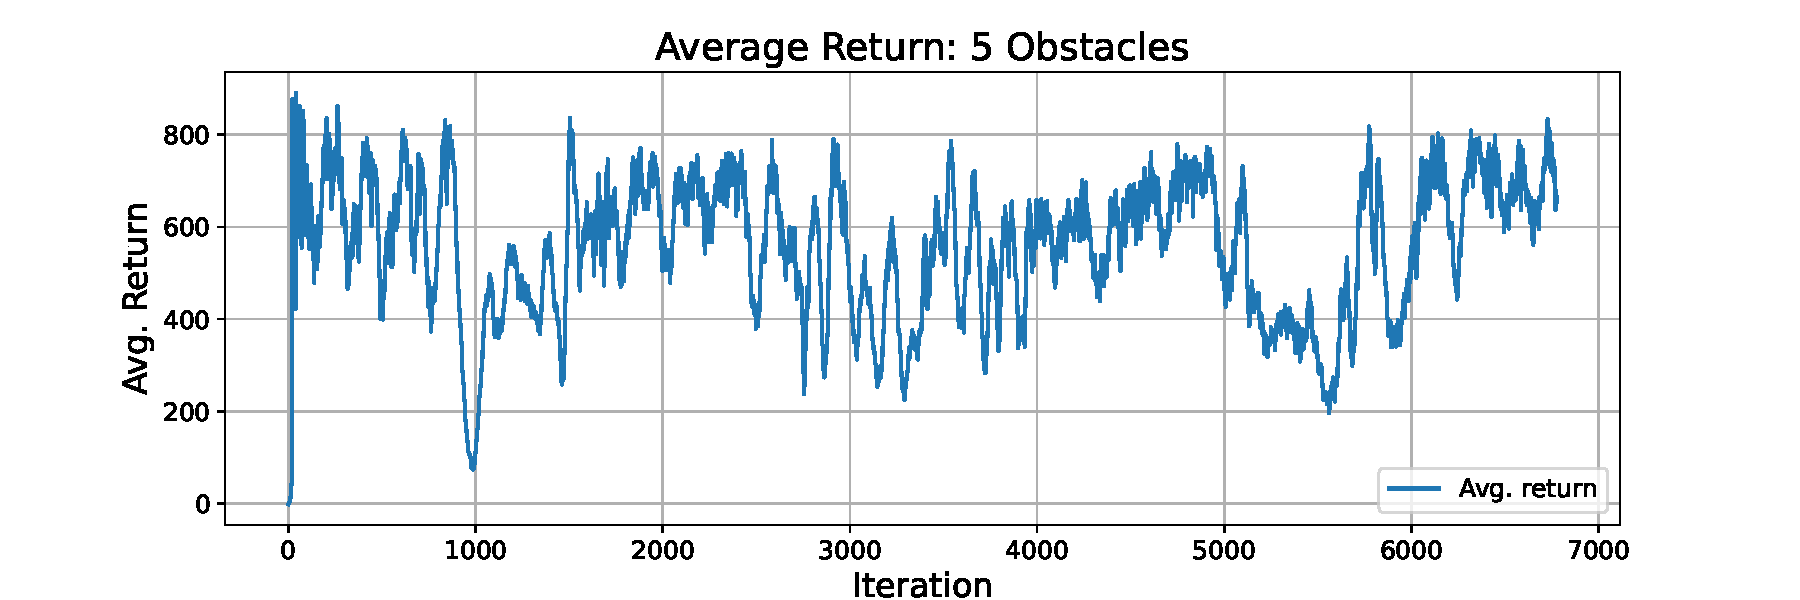
\includegraphics[width=0.99\textwidth]{figures/7_/3DCarModel_BodyObs_NavSetup_5_NewObs_v1_reward.pdf}
        \label{fig:5_obst_nav_rew}
    \end{subfigure} \\
    \begin{subfigure}[b]{\textwidth}
        \centering
        \captionsetup{justification=centering}
        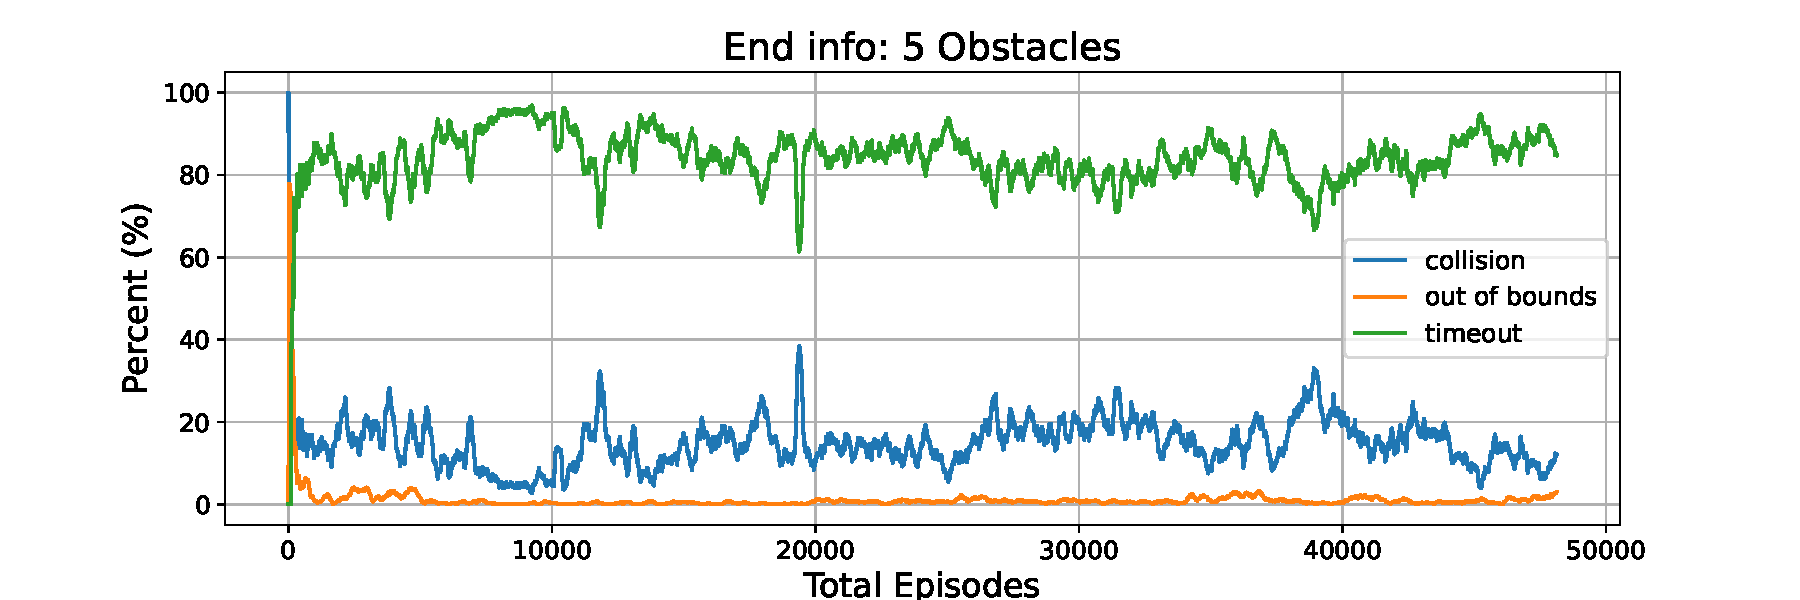
\includegraphics[width=0.99\textwidth]{figures/7_/3DCarModel_BodyObs_NavSetup_5_NewObs_v1_end_info.pdf}
        \label{fig:5_obst_nav_end}
    \end{subfigure} 
    \caption{Training with 5 obstacles. The best model is selected at 1498 iterations, with an average return of 720 and timeout rate of $94.8\%$.} %3150
    \label{fig:7_train_nav_5_obst}
\end{figure}
Once again, we observe from the figure a similar pattern for the return in the first 1000 iterations. However, unlike the 3-obstacle case, we recognise that the environment is indeed more difficult, resulting in a more complex optimisation space that causes higher fluctuations in the accumulated rewards when the agent explores different trajectories. This is also more pronounced due to the longer episode times, such that if a policy does well to reach the goal it will accumulate significantly more rewards than one that does decent but does not reach goal as closely or as often.

Another promising feature of this training plot is that the timeout rates are consistently higher than for the 3-obstacle case, even when the reward is high. The reason for this is quite indirect, though will be discussed later in \cref{subsec:9_sparse_rewards}.
Keeping this optimistic perspective, we can then move on to 9-obstacles.


\subsection{9 Obstacles}
\label{subsec:7_9_obstacles}
The most difficult environment of the training process consists of 9 obstacles in an $20\times10$ environment. Accounting for the quadrotor and goal -- a 6m spacing as seen in  -- the effective area for this obstacles is an $8\times10$ square, or an obstacle every metre for 8m. 
For perspective, we provide two images in \cref{fig:7_9_obst_and_flat_png}. 
\begin{figure}[htb]
    \centering
    \begin{subfigure}[b]{0.26\textwidth}
        \centering
        \captionsetup{justification=centering}
        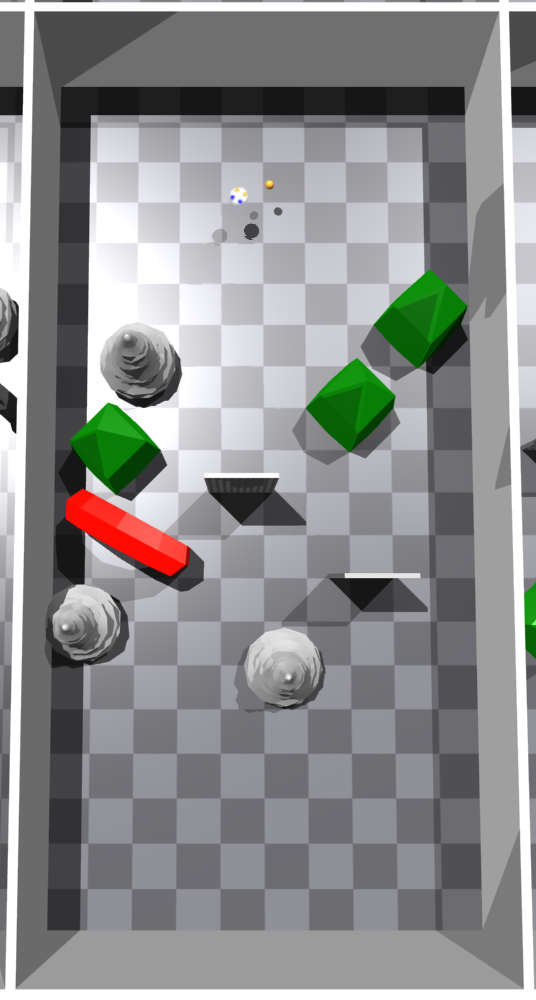
\includegraphics[width=0.99\textwidth]{figures/7_/7_9_obst.png}
        \caption{9 obstacles are placed from along $x \in [-4,4]$.}
        \label{fig:9_obst_png}
    \end{subfigure}
    \hfill
    \begin{subfigure}[b]{0.71\textwidth}
        \centering
        \captionsetup{justification=centering}
        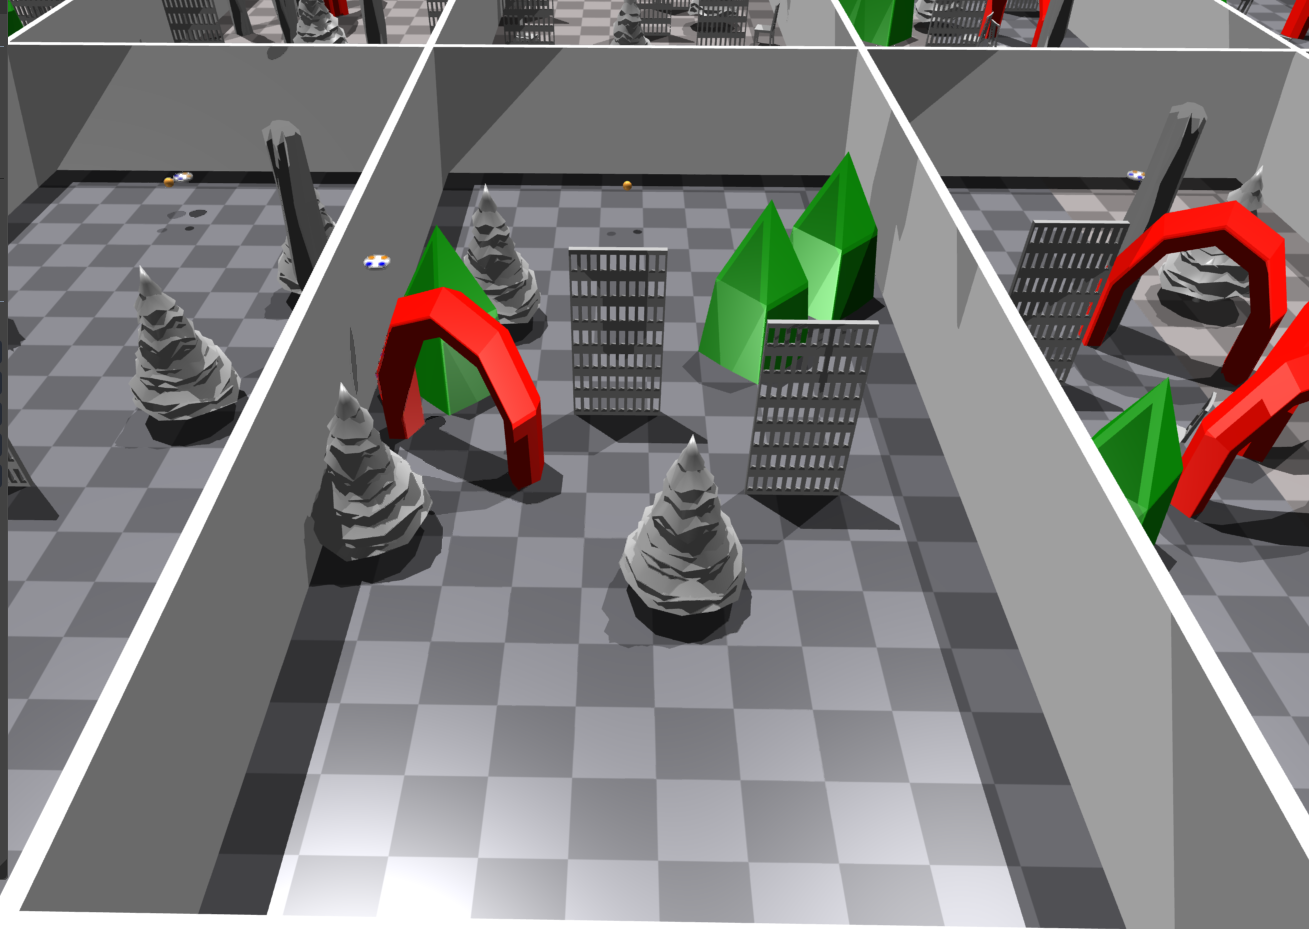
\includegraphics[width=0.99\textwidth]{figures/7_/7_9_obst_flat.png}
        \caption{Agent must display collision avoidant properties to pass.}
        \label{fig:9_obst_flat_png}
    \end{subfigure} 
    \caption{An example environment with 9 obstacles, with size $20\times10$.}
    \label{fig:7_9_obst_and_flat_png}
\end{figure}

Following the same idea for the 5 obstacle case, we provided ample time for policy training and kept the episode length $T$ the same to obtain the results in  \cref{fig:7_train_nav_9_obst}.
\begin{figure}[htb]
    \centering
    \begin{subfigure}[b]{\textwidth}
        \centering
        \captionsetup{justification=centering}
        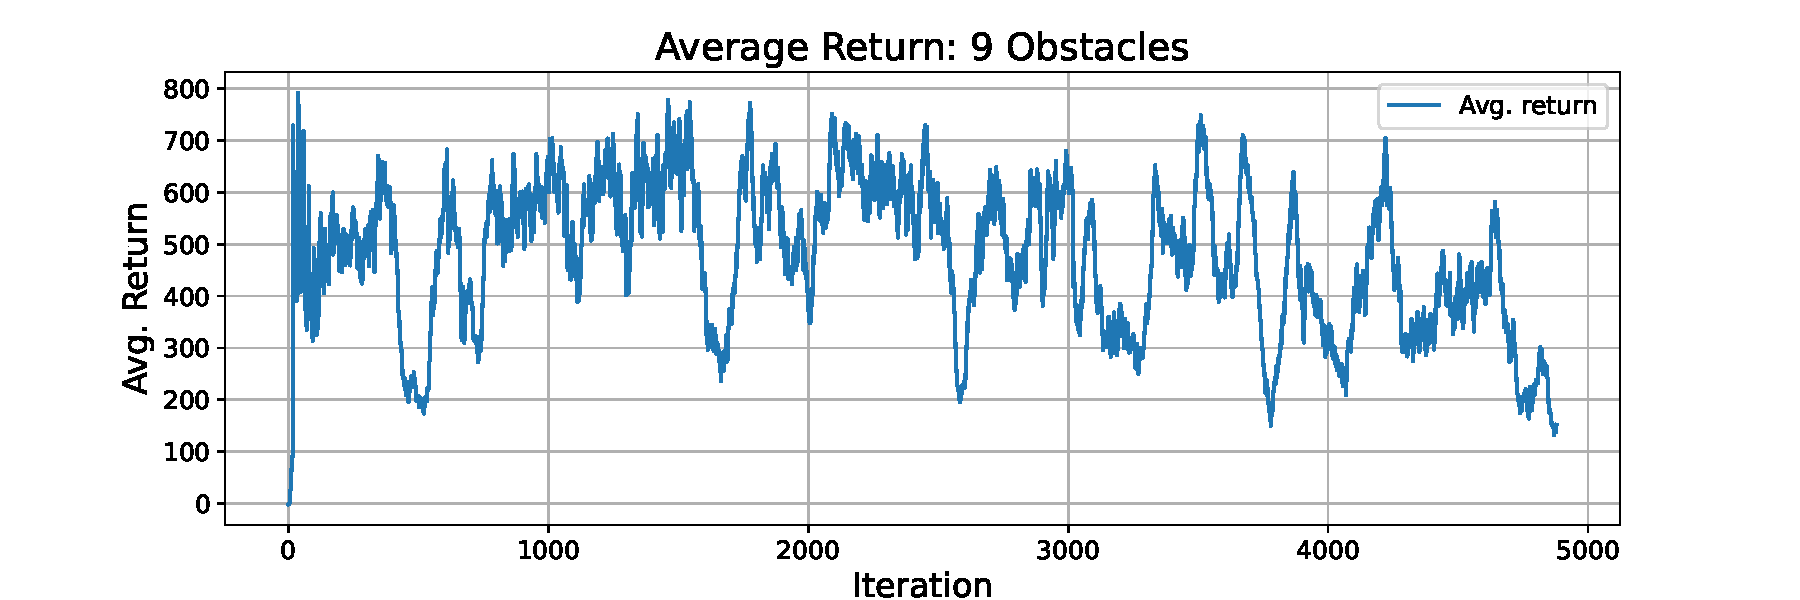
\includegraphics[width=0.99\textwidth]{figures/7_/3DCarModel_BodyObs_NavSetup_9_NewObs_EnvSpace10_last3150_v1_reward.pdf}
        \label{fig:9_obst_nav_rew}
    \end{subfigure} \\
    \begin{subfigure}[b]{\textwidth}
        \centering
        \captionsetup{justification=centering}
        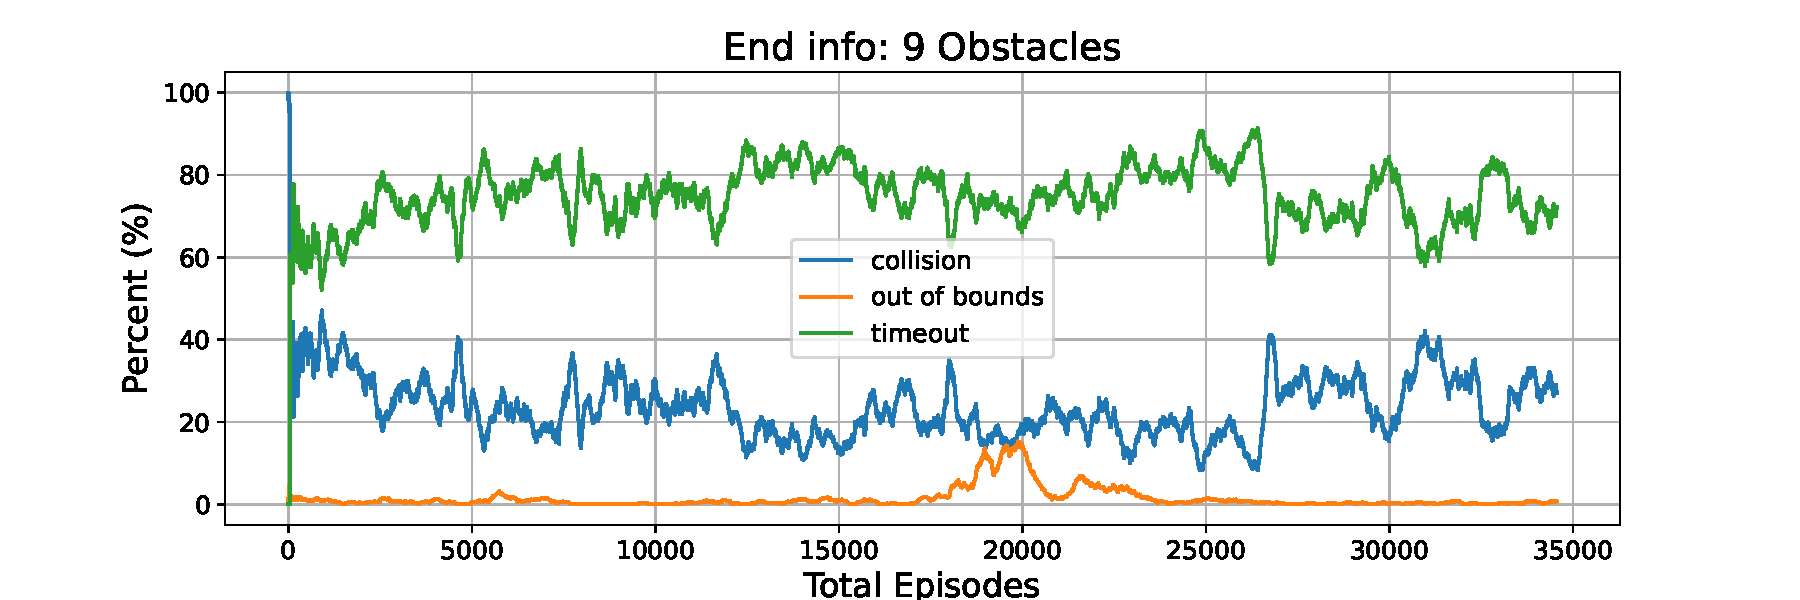
\includegraphics[width=0.99\textwidth]{figures/7_/3DCarModel_BodyObs_NavSetup_9_NewObs_EnvSpace10_last3150_v1_end_info.pdf}
        \label{fig:9_obst_nav_end}
    \end{subfigure} 
    \caption{Training with 9 obstacle. The best model is selected at 3500 iterations, with an average return of 700 and timeout rate of $84.7\%$. }
    \label{fig:7_train_nav_9_obst}
\end{figure}
Here, we see that the average return follows an upwards trend to about 1500 iterations, which reflects the difficulty of the environment as the agent takes much longer time to fine-tune its behaviour. Interestingly, we see that this trend also applies to the timeout rate but only to about 1000 iterations. This suggests that the rewards for collision avoidance and goal-reaching are aligned up some degree, but at some point, the rewards motivate the agent to learn risky behaviour -- prioritising to reach goal in situations where it could be more careful.

However, after extensive sampling, we see that the agent policy begins to learn very promising collision avoidance attributes between iterations $3200 \sim 3600$, where we select our best model at 3500 iterations. In this situation, we also note that the average return varies dramatically. To reason for this, we can assume that when the agent is learning to navigate carefully, i.e. the policy is aware of state-actions pairs that cause collisions, the conservative behaviour could mean reaching goal is unlikely. This is in contrast to the policy at around 1500 iterations which learned to ``consistently'' reach goal, though ironically with crashes. So in our situation, we can view the model at $3500$ iterations as having a good balance of both, where the policy has ``stumbled upon'' a favourable locally optimal solution with good navigational abilities.

The reason that conservative policies have a hard time reaching goals is also linked to the observation that collision rates are relatively high. Unfortunately, this is expected, and can be explained by the agent having to manoeuvre past more obstacles in the previous case. Moreover, due to the more cluttered nature of the environment, the agent can also experience \textit{getting stuck} in between obstacles where there is no clear way forward.
An example of this is shown in \cref{fig:7_9_obst_and_flat_png}, where we see a corner-type situation of the left side in between the tree and U-shape, and can observe a quadrotor flying. Of course, we can think that a quadrotor getting stuck in this situation is unlikely, seeing that it could go right for example. Yet, with 512 randomly generated environments, we can imagine that these corner-type situations could exist in many forms, both on the left and right side. We can also argue that after passing an obstacle on the left, the optimal path may be to turn and look to the right, but the quadrotor will not see this due to a limited field-of-view ($86\degree$) of the camera sensor. As a result, it will enter a corner situation, (and possibly pass) as the agent shown in \cref{fig:9_obst_flat_png}. 

So, from this corner situation, if the policy is conservative, an agent will lie and wait as to avoid collision. If it is more aggressive, it will enter and risk collision. Thus, on average, a policy that remains stuck in these unlikely situations will gather much less return that one that collides, and proceeds to find the goal in the next episode -- which provides an explanation to why higher timeout rates does not equal higher rewards. However, by chance, a policy that is both conservative \textit{and} can escape corner situations could appear, which is the case for our policy at 3500 iterations shown in \cref{fig:9_obst_flat_png}.


\section{Evaluating the Learned Navigation Policy}
\label{sec:7_evaluating_policy}

With a policy selected from the curriculum, we can now evaluate its performance in the form of standardised tests in known and unknown environments, along with assessing its robustness to noise.
For the known environments, we aim to present three variations of the environment with an increasing degree of clutter, while for unknown environments we increase the environment size.
From this, we should be able to gauge its overall performance and more interestingly its ability to generalise to unseen domains and uncertainty.

\subsection{Known Environments}
For the known environments, we test the agent in an environment of size $[20, 10]$, where we increase the number of obstacles from 7 to 12, as shown in \cref{tab:7_known_tests}. Unlike training, we use a non-randomised environment such that we can visualise the behaviour of different policies in a standardised context. We then run our policy in each environment for 1000 episodes and document the episode end label.
\begin{table}[htb]
    \centering
    \begin{tabular}{||c|c|c|c|c|c|c||}
    \hline
    Level & No. of & Space per obst. & Timeouts & Collisions & Out. of & Timeout \\  
     & obstacles & (m$^2$ / obst.) & & & bounds & rate (\%) \\\hline\hline
    Easy    & 7  & 11.4   & 980 & 21 & 0 &  97.9 \\\hline
    Medium  & 9  & 8.89   & 967 & 33 & 2 &  96.5 \\\hline
    Hard    & 12  & 6.67  & 771 & 230 & 0 & 77.0 \\\hline
    \end{tabular}
    \caption{For the known environments, we evaluate the agent's response to a variation in the cluttered-ness of the environment. We choose an environment size of $[20, 10]$, which is an $8\times 10$ or 80m$^2$ effective obstacle area.}
    \label{tab:7_known_tests}
\end{table}

From the table, it is clear that the reinforcement learning agent is extremely successful in navigating \textit{known} cluttered environments, though its performance is bounded by the available space to some extent. Compared to our expectations from training, these are certainly impressive results, given that the timeout rate for the 9-obstacle environment is 96.5\% timeout rate compared to $84.7\%$ in \cref{fig:7_train_nav_9_obst}. An explanation for why we did not see such a high timeout rate in training is because the end information plots are \textit{averaged} over 1000 episode ends. Following this, an indication which shows very good collision avoidance in the policy is that the \textit{slope} of the timeout rate is very high at 3500 iterations -- indicating a much higher timeout rate under the current policy, which pushes the average up. Otherwise, it could also be that the environments in training are randomised, which suggests that the environments used for testing are ``too easy''. To see for ourselves, we can look at Figures \ref{fig:7_easy}, \ref{fig:7_medium} and \ref{fig:7_hard}.
\begin{figure}[!htbp]
    \centering
    \makebox[\textwidth]{
    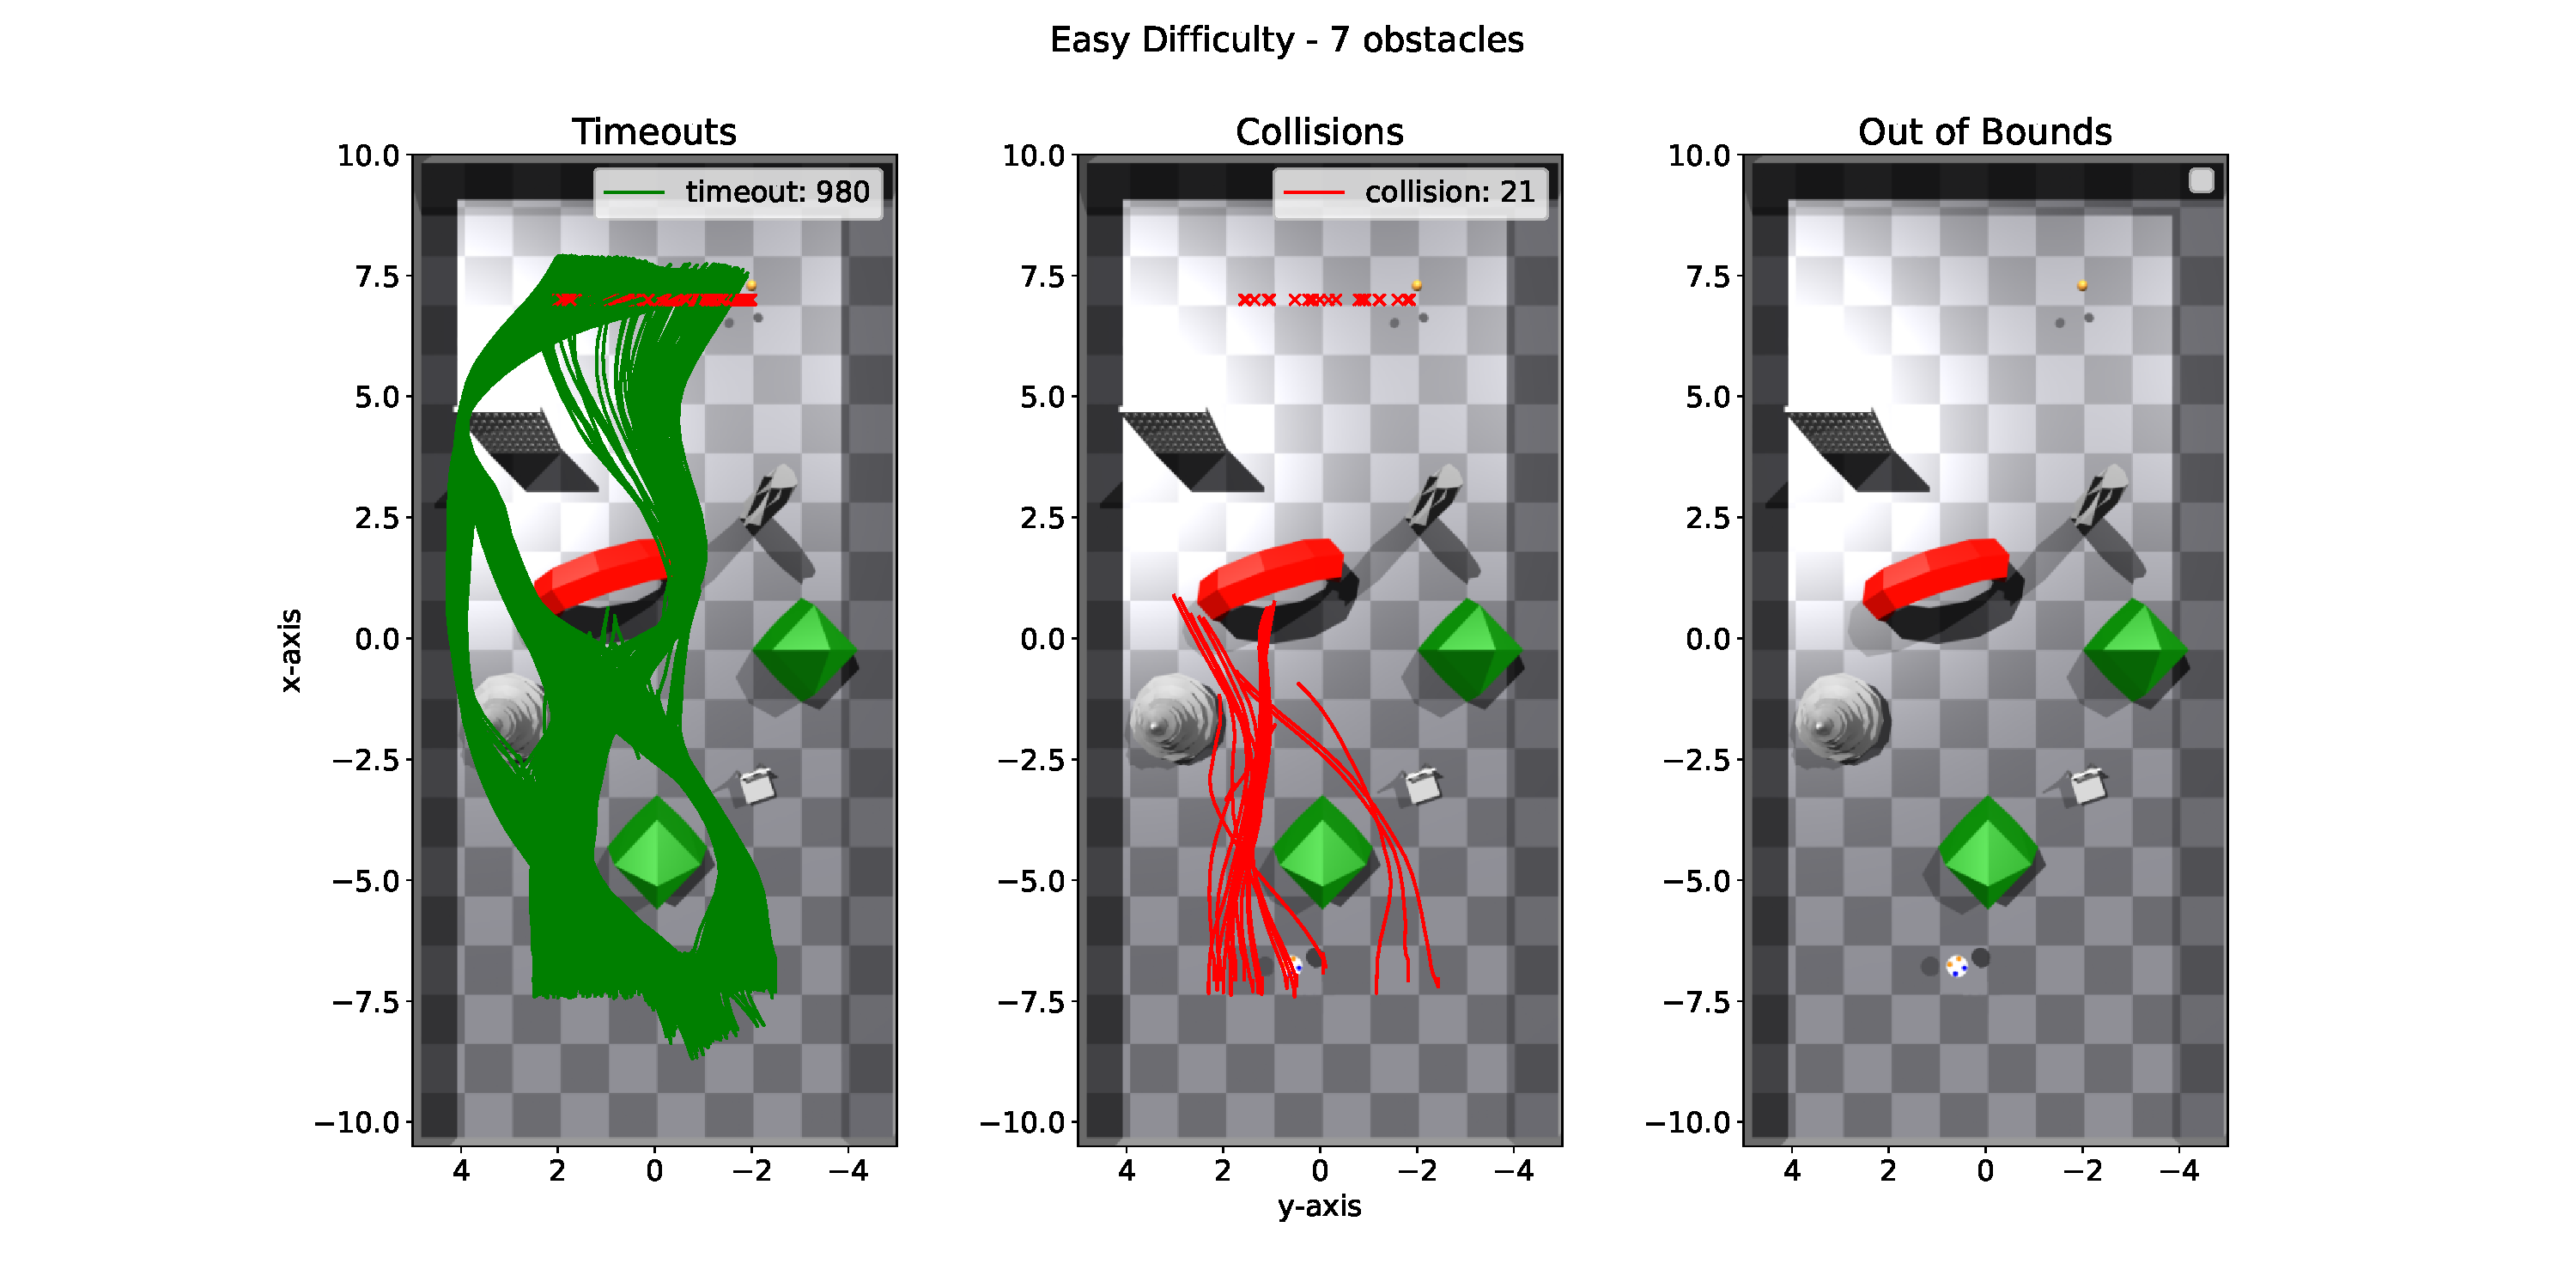
\includegraphics[width=1.2\textwidth]{figures/7_2/easy.pdf}
    }
    \caption{The environment with an easy difficulty with a timeout rate of 97.9\%. There are 7 objects in this environment, where multiple are placed in the the agent's line-of-sight so that collision-avoidance is necessary for all trajectories. Despite this, openings are relatively spacious compared to difficult environments.}
    \label{fig:7_easy}
\end{figure}
\begin{figure}[!htbp]
    \centering
    \makebox[\textwidth]{
    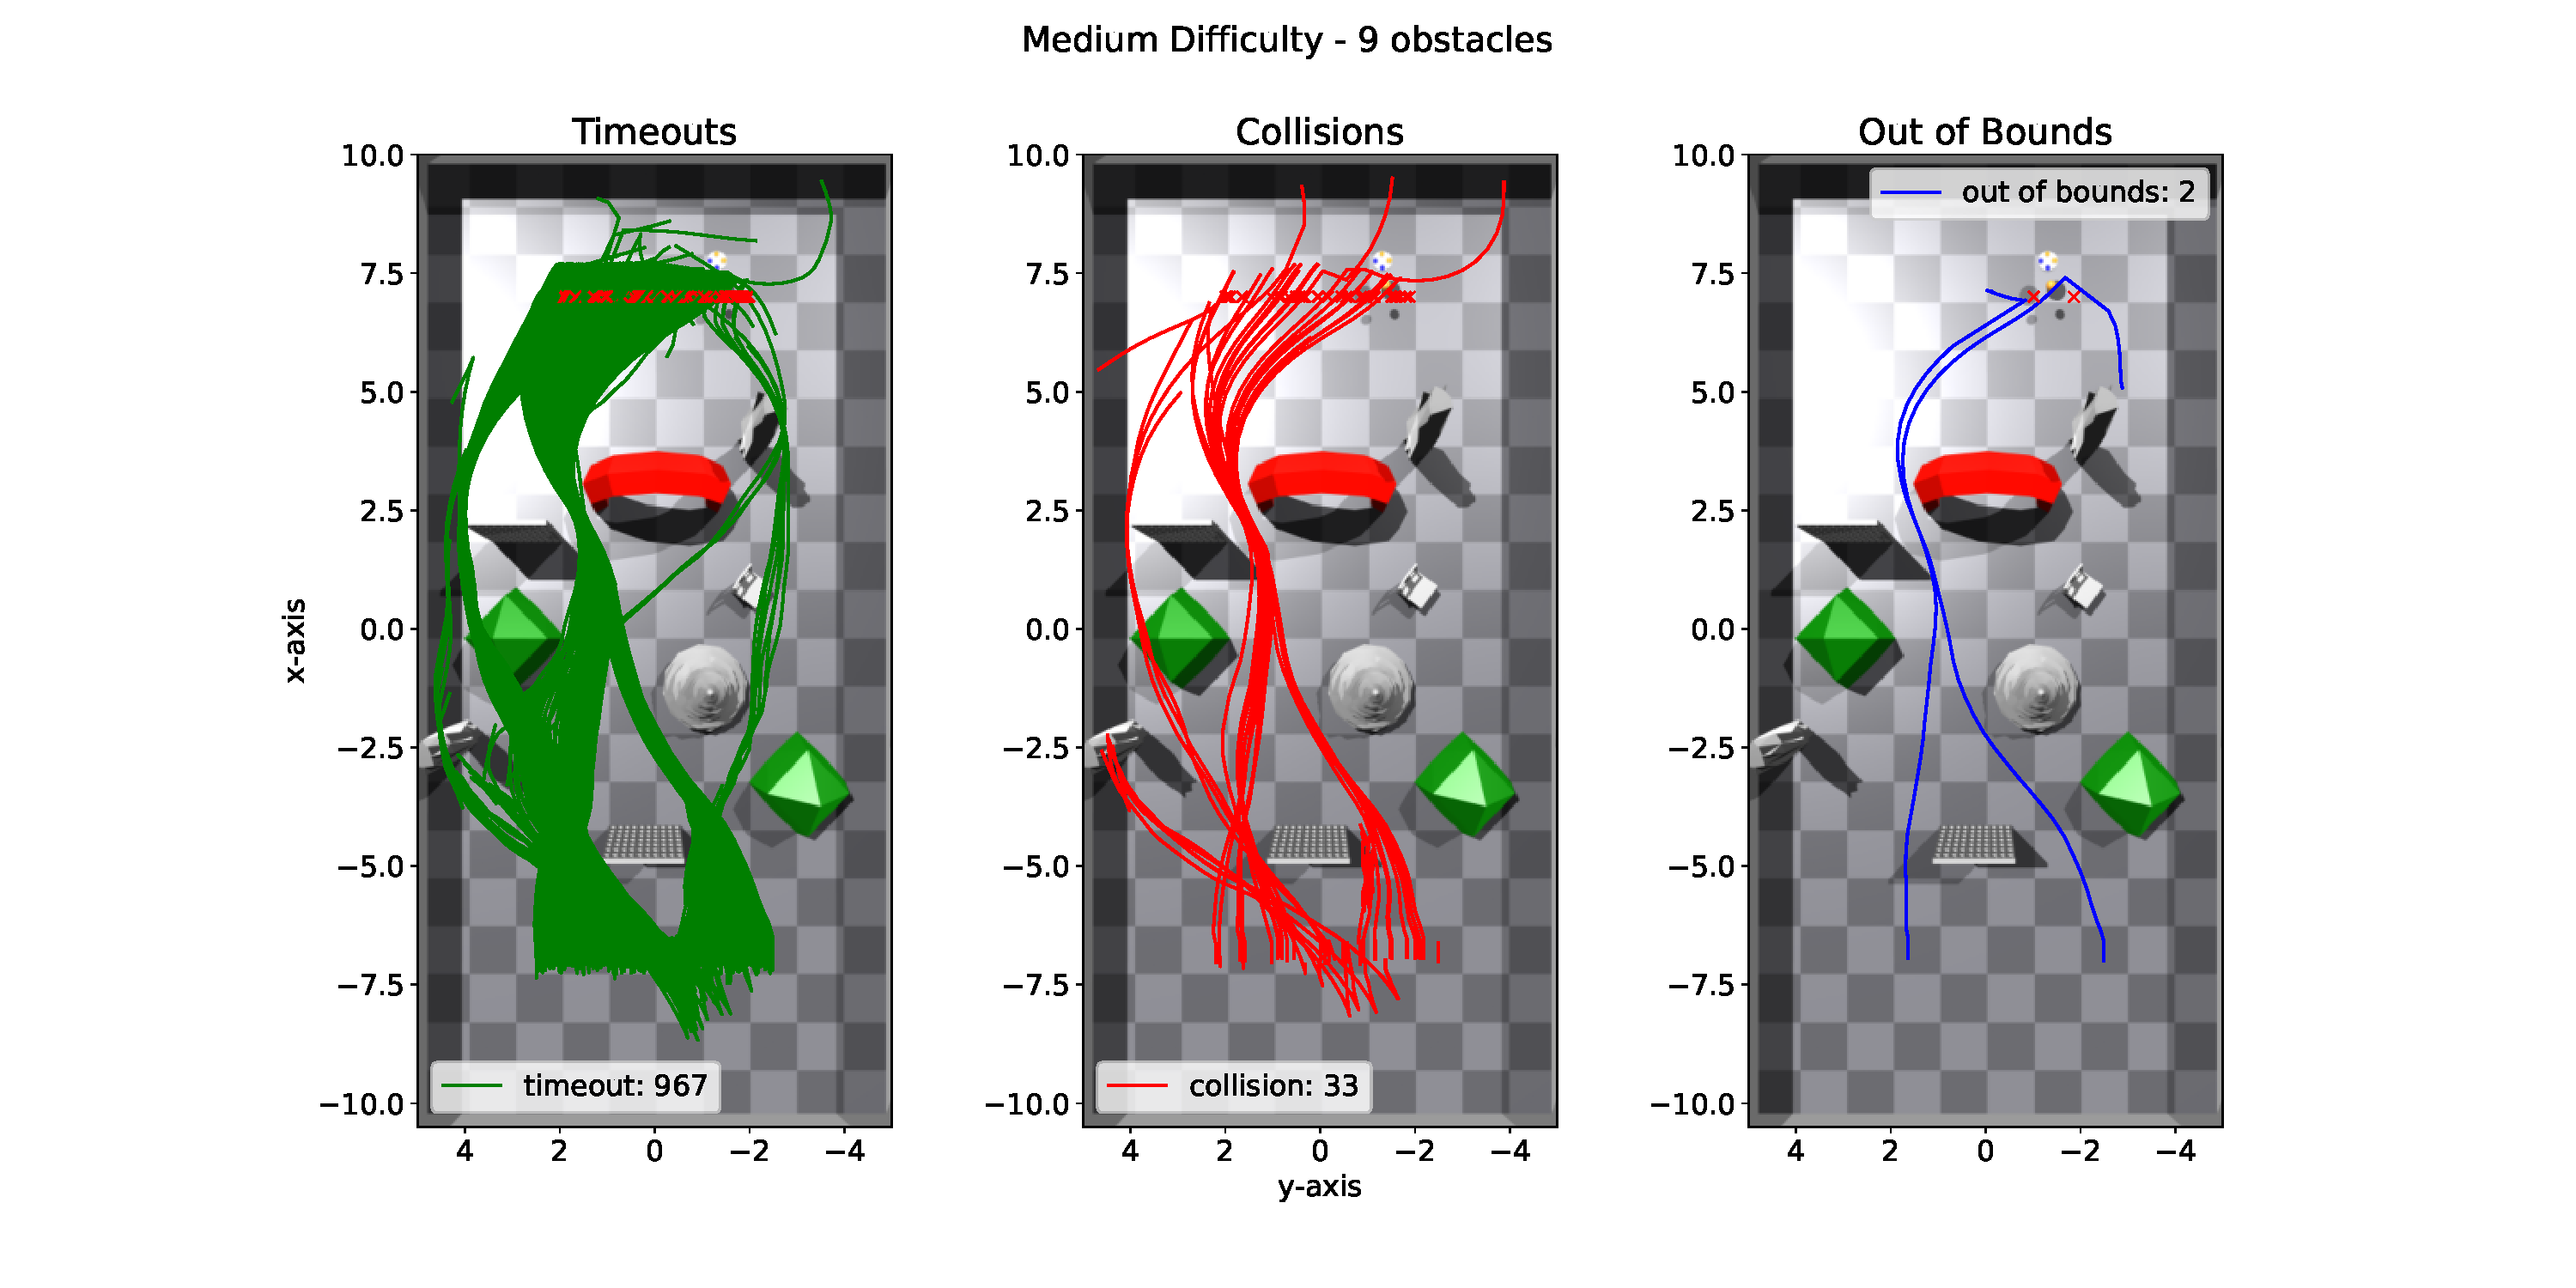
\includegraphics[width=1.2\textwidth]{figures/7_2/medium.pdf}
    }
    \caption{The environment with an medium difficulty with a timeout rate of 96.5\%. 9 obstacles are placed so to reduce the size of openings and increase the average number of obstacles to pass per trajectory. This results in a large trajectory distribution and roughly 50\% more collisions than the easy environment.}
    \label{fig:7_medium}
    \makebox[\textwidth]{
    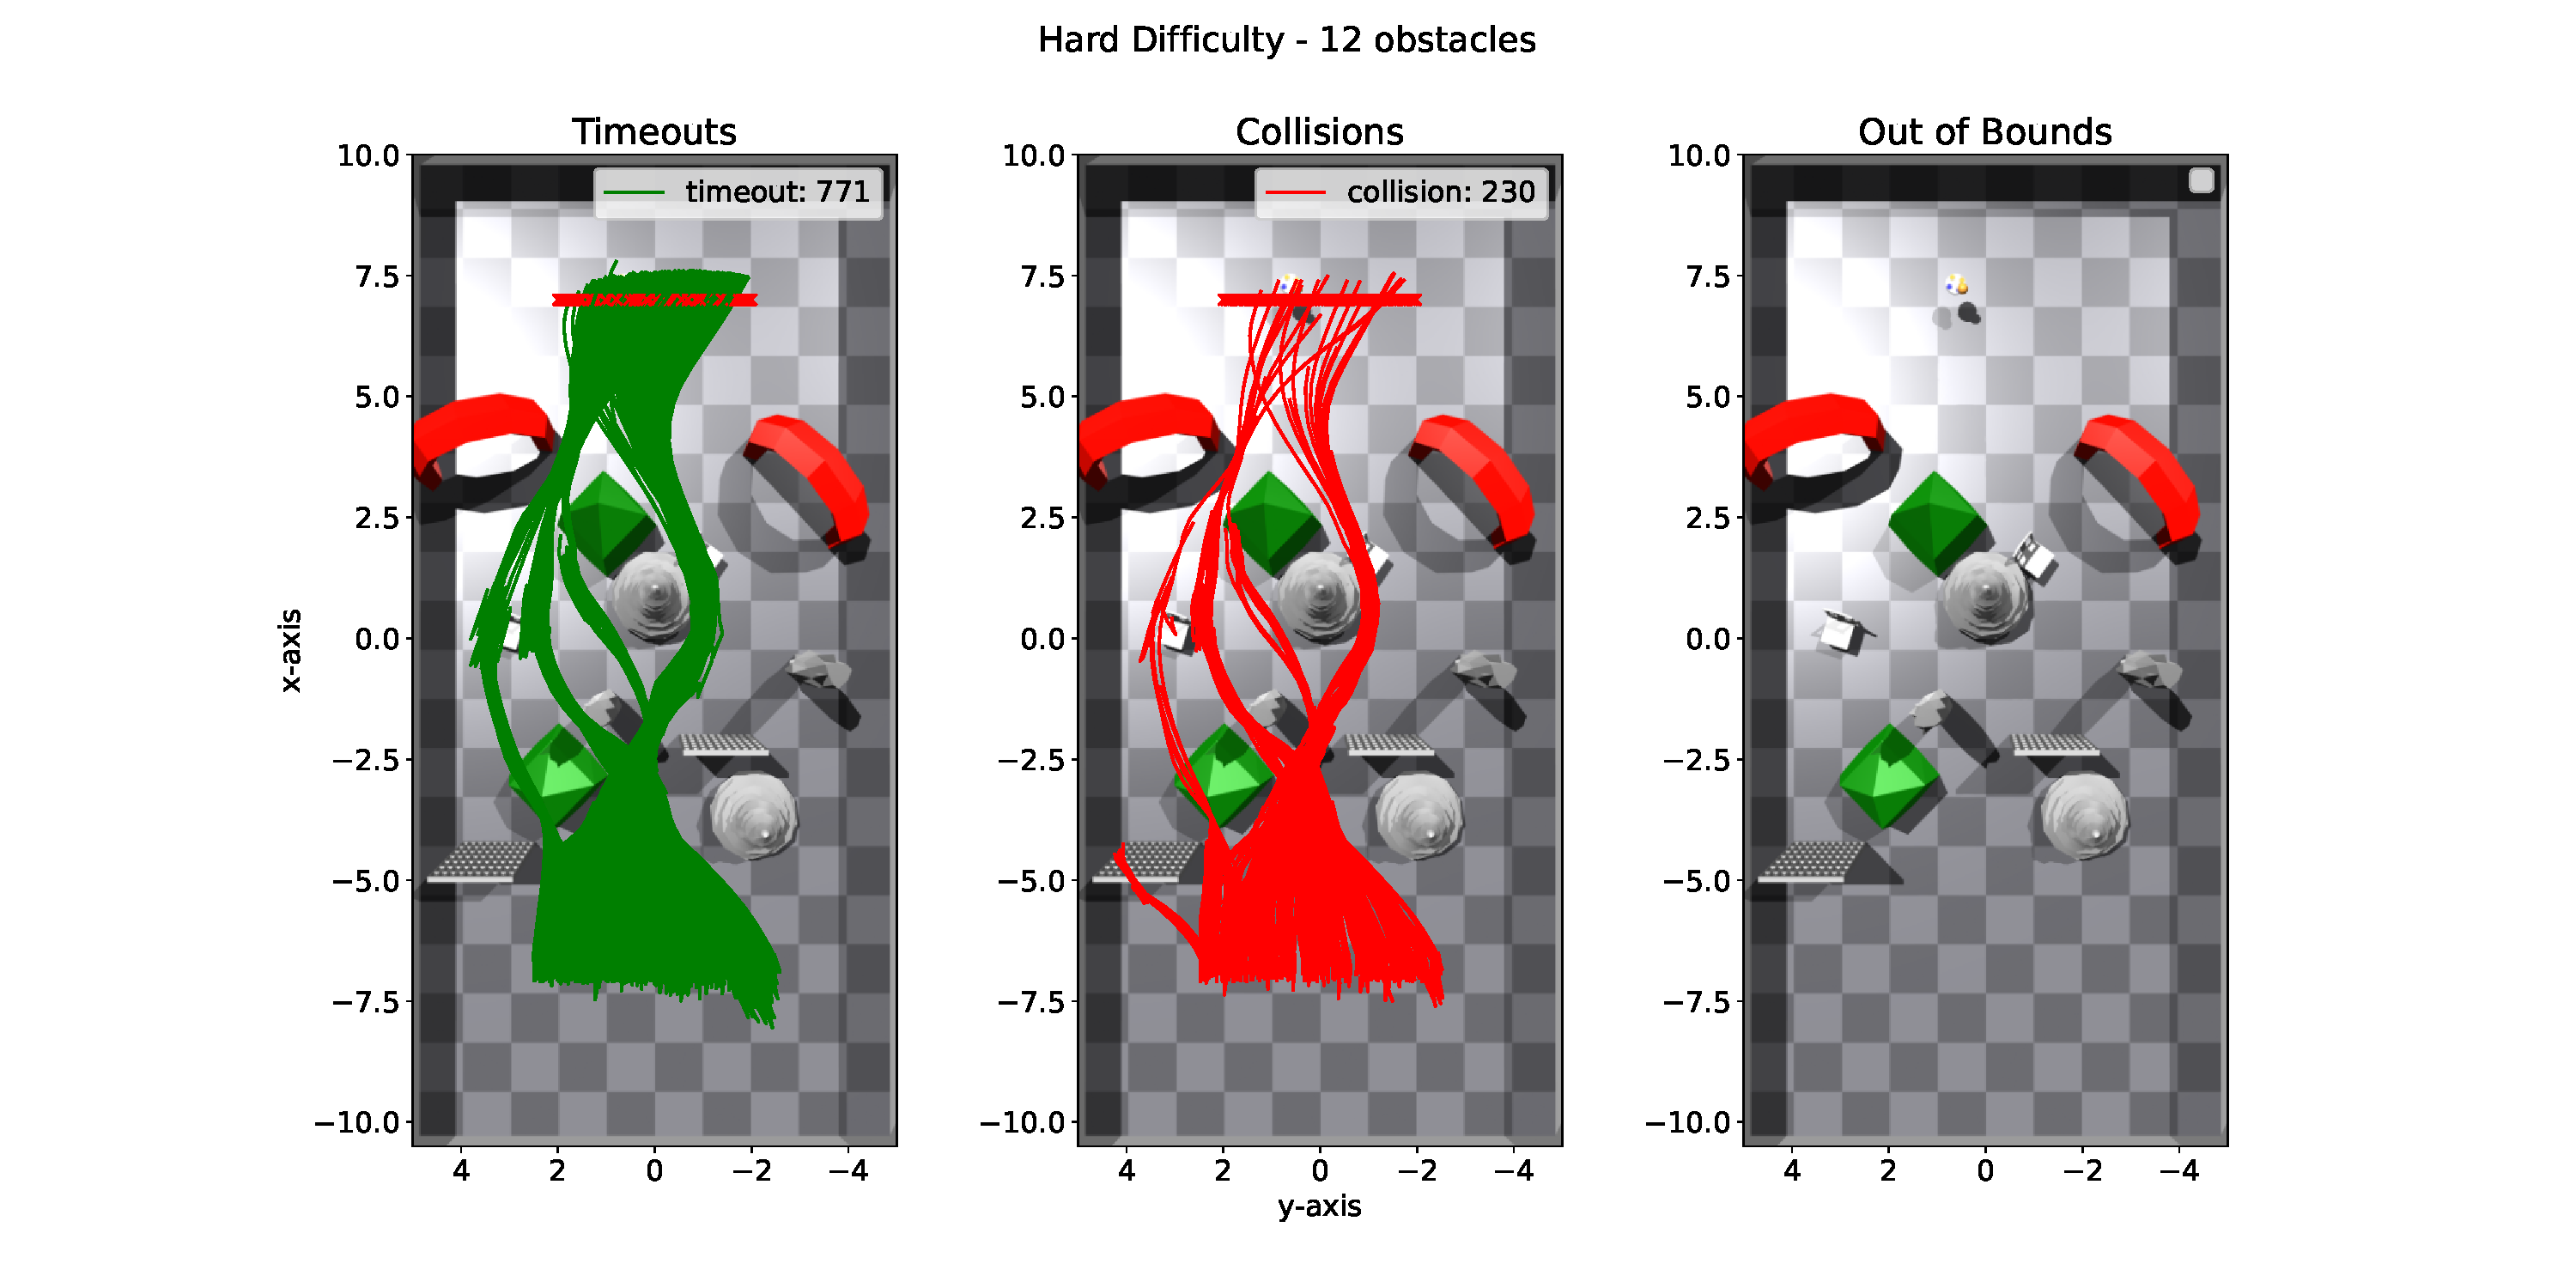
\includegraphics[width=1.2\textwidth]{figures/7_2/hard.pdf}
    }
    \caption{The environment with an hard difficulty with a timeout rate of 77.0\%. We test the agent's leftward bias by reduce opening sizes further on the left size. Turns are also much sharper, which induces many pass-by collisions.}    
    \label{fig:7_hard}
\end{figure}

From these, it is evident that the degree of clutter is increasing, but also the number of obstacles that the agent is forced to avoid in order to reach goal. For the easy environment, we see that any chosen trajectory must avoid on average 3-4 obstacles, which increases to roughly 4 in the medium environment, and to roughly 5 in the most dense environment. We also note that the size of the openings along the agent trajectories significantly decreases for each environment.
However, we do recognise that there are no corner-like situations, where we intentionally trap the quadrotor.
From these observations, it is plausible that the existence of these corner-situations account for the majority of collisions, since we see that the policy is more than capable of navigating past 4 obstacles with a timeout rate of $96.5\%$.

To look more into the detail of the quadrotor behaviour, we observe that the policy is heavily biased to making left-turns, despite it being unnatural or completely unnecessary. This can be seen the easy plot, where after avoiding the first pyramid the simple-u in the center, the quadrotor decides to turn extensively to the left despite being able to move straight towards goal. The result of this bias is of course collisions, as we can see in \cref{fig:7_easy}, where all collisions are caused by forcing entry through the tight space between the simple-u and the pine tree.

Another, quite unexpected, behaviour that the quadrotor has learned is to be able to \textit{reverse}. We see when the quadrotor spawns directly in front of the simple pyramid, quite a few of the trajectories first \textit{go backwards}, before reaching goal and being marked as green. This behaviour is unexpected because we provide no rewards for reversing, except for a $<1$m from obstacle penalty. In fact, we actually provide penalties for reversing -- thus actually discouraging it. So surprisingly, we see that the this behaviour has been learned completely learned through sampling, where the policy decides that if its vision is completely blocked by an obstacle -- it should reverse in order to reach goal.

The obvious consequence of this behaviour however, is that it induces potential crashes due to blindness. This is most visible in \cref{fig:7_hard}, where the quadrotor collides with the chair on the left side after reversing due to the tight placement of obstacles.
Perhaps unclear, in \cref{fig:7_medium}, some of the collisions are a result of the quadrotor reaching goal, but reversing slightly to adjust its placement. However, sometimes this results in excessive reversing, to which the the quadrotor collides with the wall. 

Another common reason why collisions occur is not due to the necessity of collision avoidance, but rather to an uncareful approach to goal. As we see in \cref{fig:7_medium}, many trajectories do reach goal but seem to result in collisions. By doing a quick investigation, it can be seen that these are either from reversing or from descending.
The need for descending is a result of the quadrotor attempting to fly as high as possible during the obstacle course, as most obstacles are become thinner with height, while the goal is between $\z \in [0.5, 1.5]$. Yet, though it is effective to fly above these obstacles, its decent is still imperfect, which results in collisions either with the ground near goal, or with e.g. a chair in \cref{fig:7_hard}. 

However, the two most dominating causes for collisions is a result of \textit{pass-by} collisions and \textit{tight} collisions. The pass-by collisions can be described as when the agent is forced to fly around an obstacle when approaching it parallelly, while the tight collisions are when the quadrotor aims to enter a narrow opening, but executes it imprecisely. Examples of these are seen in \cref{fig:7_hard}, where the agent crashes with the fence, simple stone and pyramid in the early center and the pyramid at the end. To identify possible reasons why these occur, we can imagine that in pass-by collisions, just about when the quadrotor passes an obstacle, it disappears from its field-of-view. Normally this is fine, but when the quadrotor approaches it parallelly, the obstacle is so close that when the quadrotor turns or descends while moving forward, a collision can occur. Tight collisions are very related, as they require an agent to pass directly through the center from a perpendicular approach. If coming from an angle, this requires turning through the center but may result in a pass-by collision.
We can link these two through the concept of \textit{space}, which we discuss in the next section.


\subsubsection{Effects of Obstacle Placement}
As mentioned, one of the most significant differences between the hard environment compared to the easy and medium ones is not the number of obstacles, but rather the availability of space when passing obstacles. We see this quite clearly in \cref{fig:7_hard}, where the agent chooses among four very tight trajectories on the left, and does not exploit the open space on the right. This is of course a result of its learned behaviour, where it simply maps various obstacle representations in its latent space to a positive yaw rates.

We can expect that therefore, if we create an artificial corner on the left side -- i.e. obstacles tightly placed together -- we can dramatically reduce its performance as we exploit the policy's weakness. Conversely, if we facilitate navigation on the left side through slightly larger openings, we can postulate that the collision rates will significantly drop, regardless of the number of obstacles it must pass on the way.
To evaluate this theory, we perform another test on the hard environment, where we switch the simple stone (pillar) with the less obstructive chair on the left side (for reference see the out of bounds plot in \cref{fig:7_hard}). From just this modification, keeping everything else constant, we obtain the results in \cref{tab:7_hard_swapped_test}.
\begin{table}[!hbt]
    \centering
    \begin{tabular}{||c|c|c|c|c|c|c||}
    \hline
    Level & No. of & Space per obst. & Timeouts & Collisions & Out. of & Timeout \\  
     & obstacles & (m$^2$ / obst.) & & & bounds & rate (\%) \\\hline\hline
    Hard, swapped  & 12  & 6.67  & 987 & 14 & 0 & 98.6 \\\hline
    \end{tabular}
    \caption{By replacing the simple stone with the chair, we allow a larger opening in the center that significantly impacts our results. We note specifically a drop in the number of collisions, from \textit{230} down to only \textit{14} when simulating for 1000 episodes.}
    \label{tab:7_hard_swapped_test}
\end{table}
The results do confirm our hypothesis, and to a very large extent. We can also see its effect on the distribution of trajectories in \cref{fig:7_hard_swapped}.
\begin{figure}[htb]
    \centering
    \makebox[\textwidth]{
    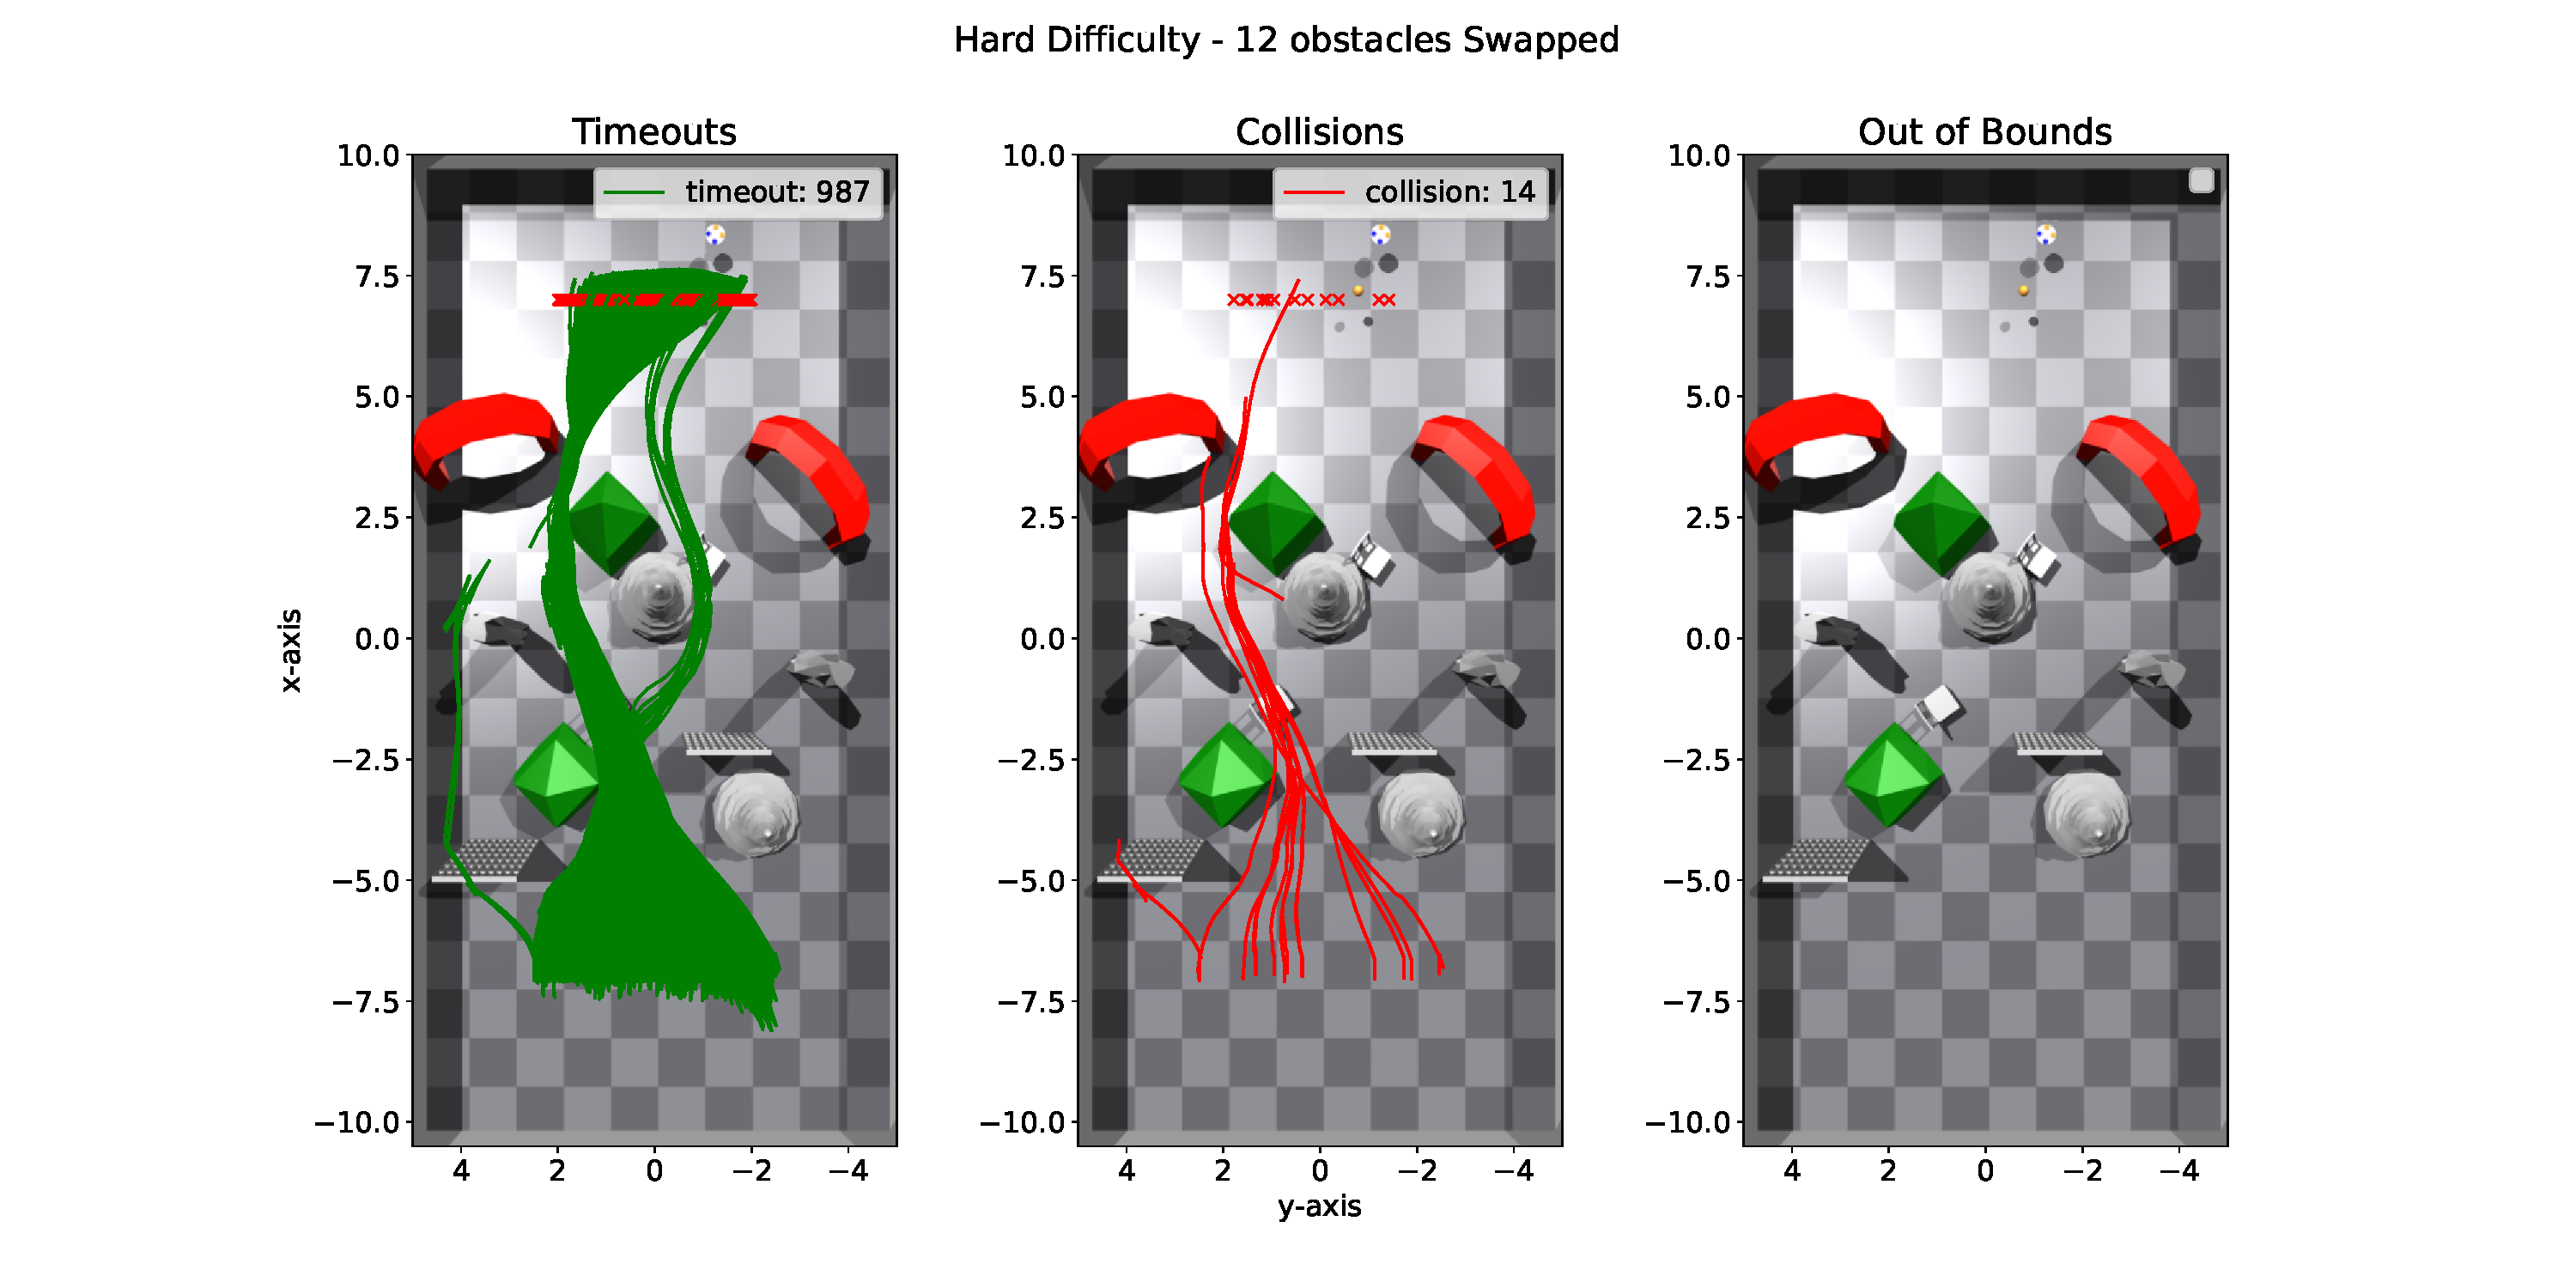
\includegraphics[width=1.2\textwidth]{figures/7_2/hard_swapped.pdf}
    }
    \caption{The hard environment where the chair on the left is swapped with the simple stone in the centre. This results in a timeout rate increase from 77.0\% to 98.6\% despite the agent having to account for the same number of obstacles.}
    \label{fig:7_hard_swapped}
\end{figure}
As a result of the switch, almost all the trajectories pass through the center opening, directly above the chair. Following this, the quadrotor is no longer forced into a position where it has to pass the end pyramid from a parallel approach, which eliminates the collision probability substantially. We can also assume that simply shifting the simple stone half a metre (half a square) to the right, we will obtain a similar result. This shows that facilitating space along an an apparent quadrotor path is more important than the number of obstacles the quadrotor has to pass. 

Of course, it will be interesting to evaluate the performance of the policy further -- blocking off paths, etc. -- though in light of the purpose of this thesis, i.e. we must remind ourselves that we are designing a policy for local motion planning in cluttered environments and not a path planner through extremely dense ones.
From a practical aspect, we can thus emphasise that it is important to weigh the strengths of a local motion planner when for example combining it with some global waypoint planner.  


\subsection{Robustness to Noise in States and Actions}
With overall very successful results, an important evaluation that must be done is one of the performance of the quadrotor when presented with uncertainty. To add noise to our quadrotor states and actions, we follow the documentation in Isaac Gym\footnote{See domain randomisation: \url{https://github.com/NVIDIA-Omniverse/IsaacGymEnvs/blob/main/docs/domain_randomization.md}} and emulate Gaussian noise $\epsilon_n \sim \mathcal{N}(1, 0.2)$ with mean of 1 and variance of 0.2, which we multiply to all quadrotor observations and actions. Multiplicative noise was chosen as opposed to additive due to the fact that we do not normalise our states directly (we leverage IsaacGym's implementation as mentioned in \cref{subsec:6_normalisation}), such that we obtain we ensure proper scaling of noise to all variables. We also ensure that the depth images are noise-free at this stage. With this added noise, we obtain the results in \cref{tab:7_noise_known_tests}.
\begin{table}[htb]
    \centering
    \begin{tabular}{||c|c|c|c|c|c|c||}
    \hline
    Level & No. of & Space per obst. & Timeouts & Collisions & Out. of & Timeout \\  
     & obstacles & (m$^2$ / obst.) & & & bounds & rate (\%) \\\hline\hline
    Noisy Easy    & 7  & 11.4   & 987 & 13 & 0 &  98.7 \\\hline
    Noisy Medium  & 9  & 8.89   & 959 & 34 & 7 &  95.9 \\\hline
    Noisy Hard    & 12  & 6.67  & 804 & 262 & 0 & 75.4 \\\hline
    Noisy Hard,    & 12  & 6.67  & 831 & 207 & 4 & 79.8 \\
    swapped & & & & & &\\\hline
    \end{tabular}
    \caption{For the noisy environments, we evaluate the agent's response to induced noise in all of the quadrotor states and actions, where each state is multiplied with $\epsilon_n \sim \mathcal{N}(1, 0.2)$. We perform this test to all known environments.}
    \label{tab:7_noise_known_tests}
\end{table}
\begin{figure}[htb]
    \centering
    \makebox[\textwidth]{
    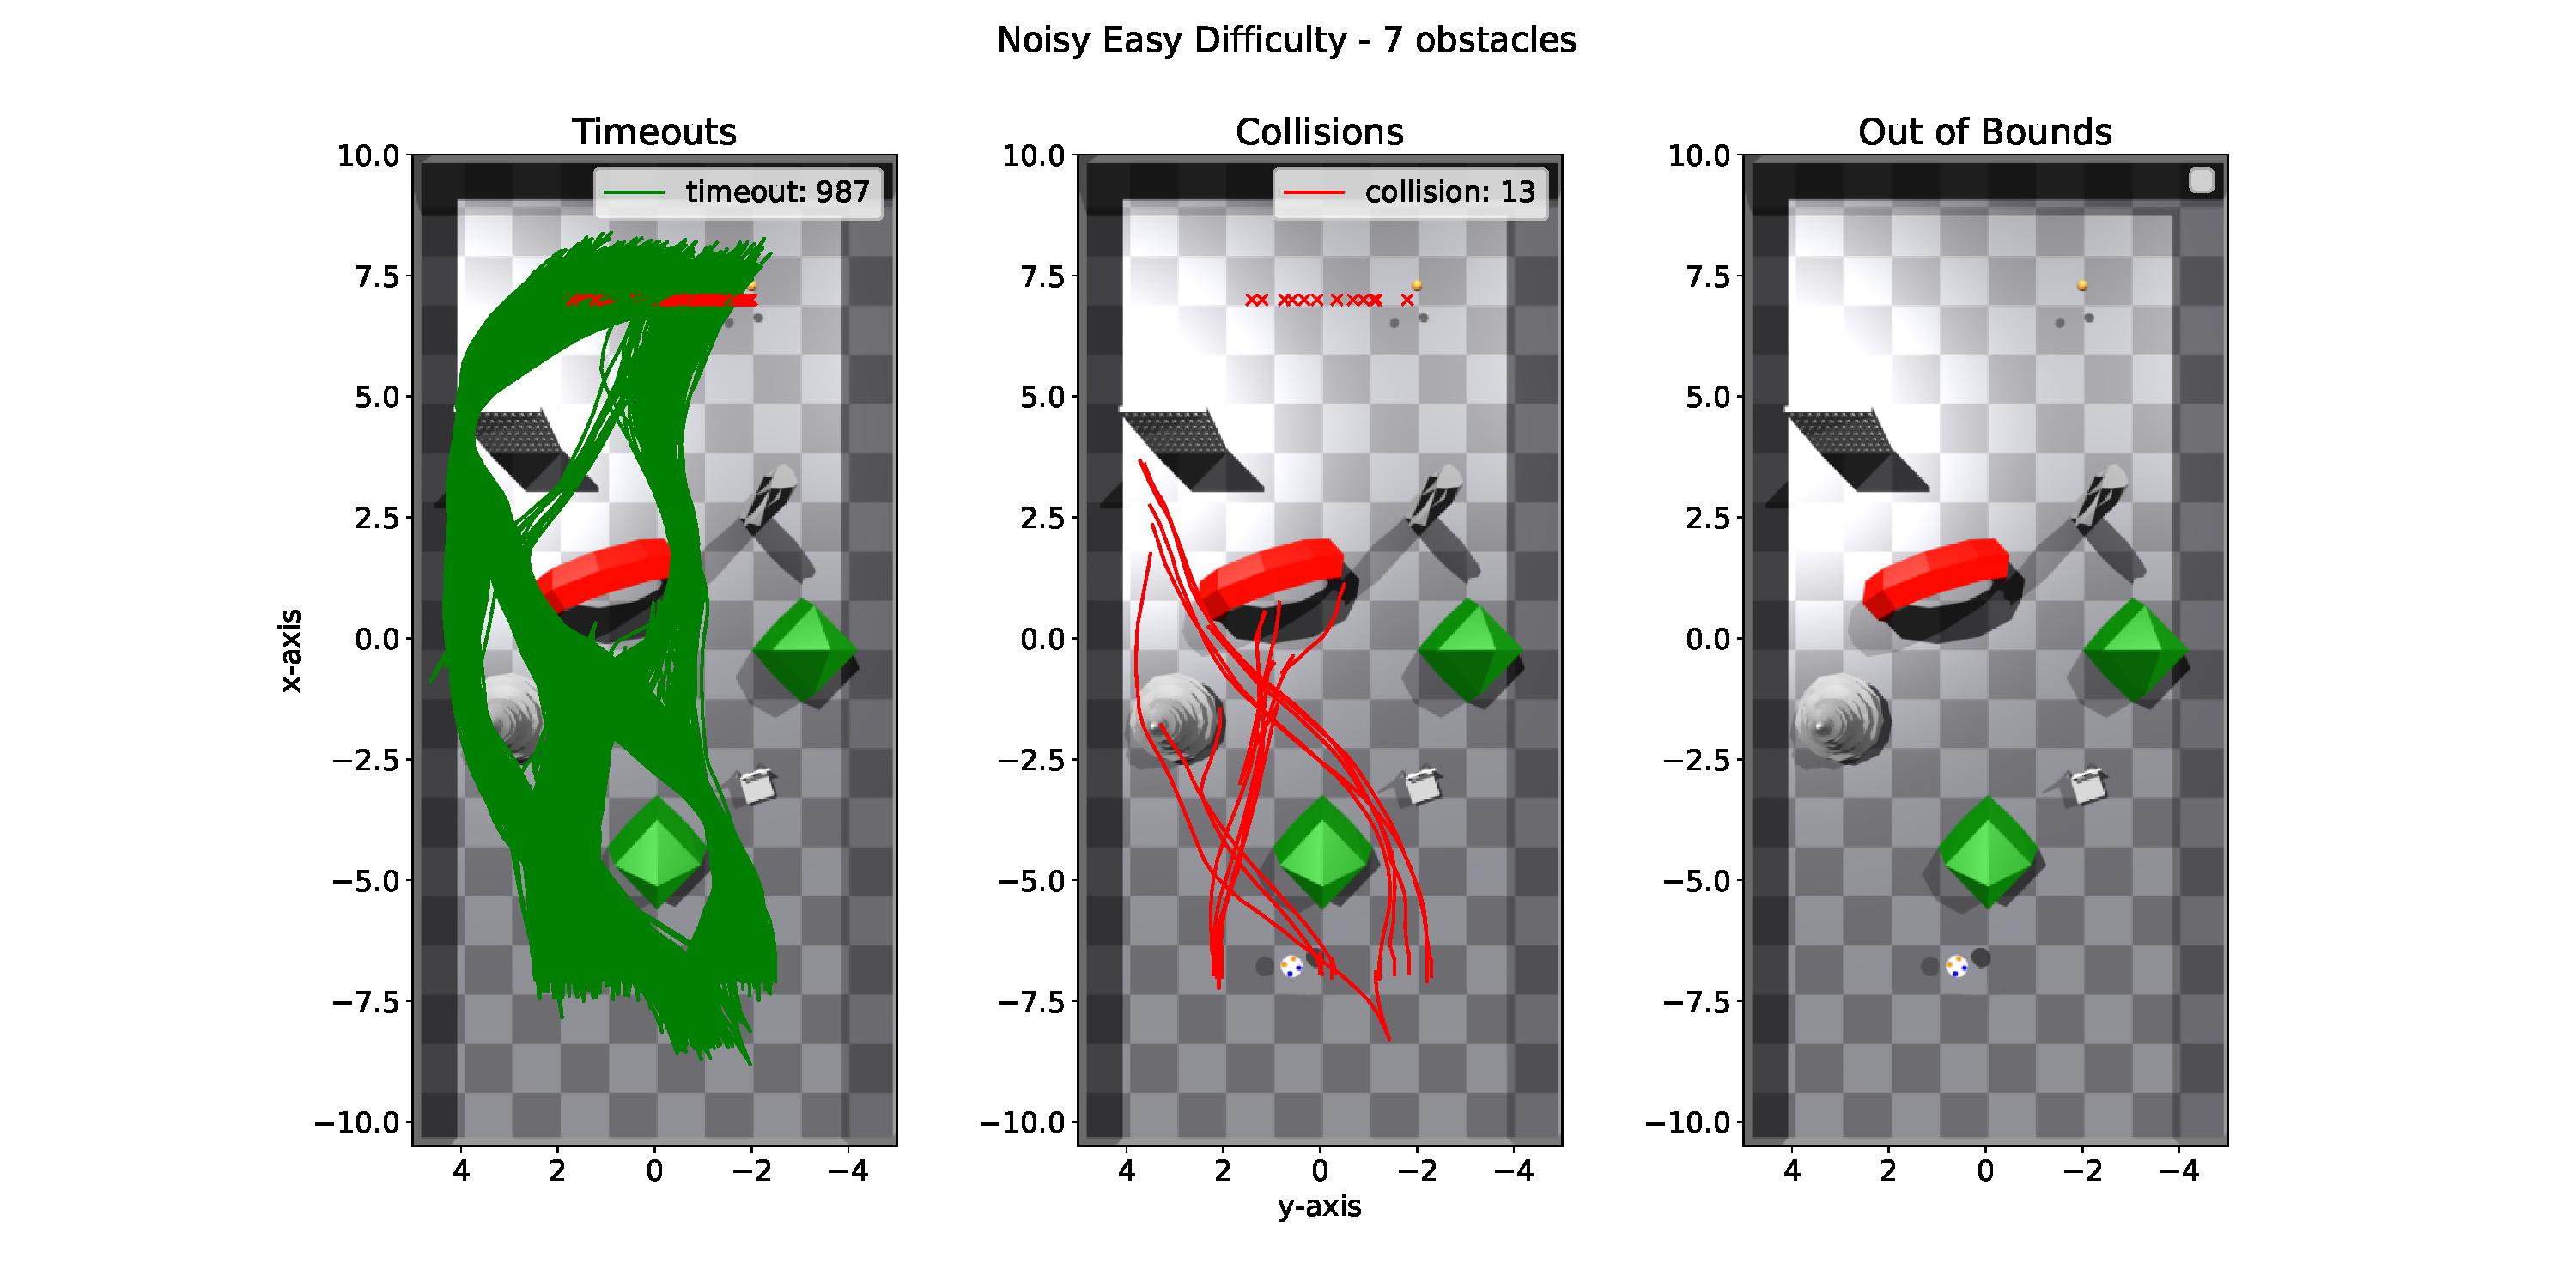
\includegraphics[width=1.2\textwidth]{figures/7_2/easy_random.pdf}
    }
    \caption{Noisy easy environment, with a timeout rate of 98.7\%. The significance of noise is not as prevalent in the collision statistics for open-space environments.}
    \label{fig:7_easy_random}
\end{figure}
\begin{figure}[htbp]
    \centering
    \makebox[\textwidth]{
    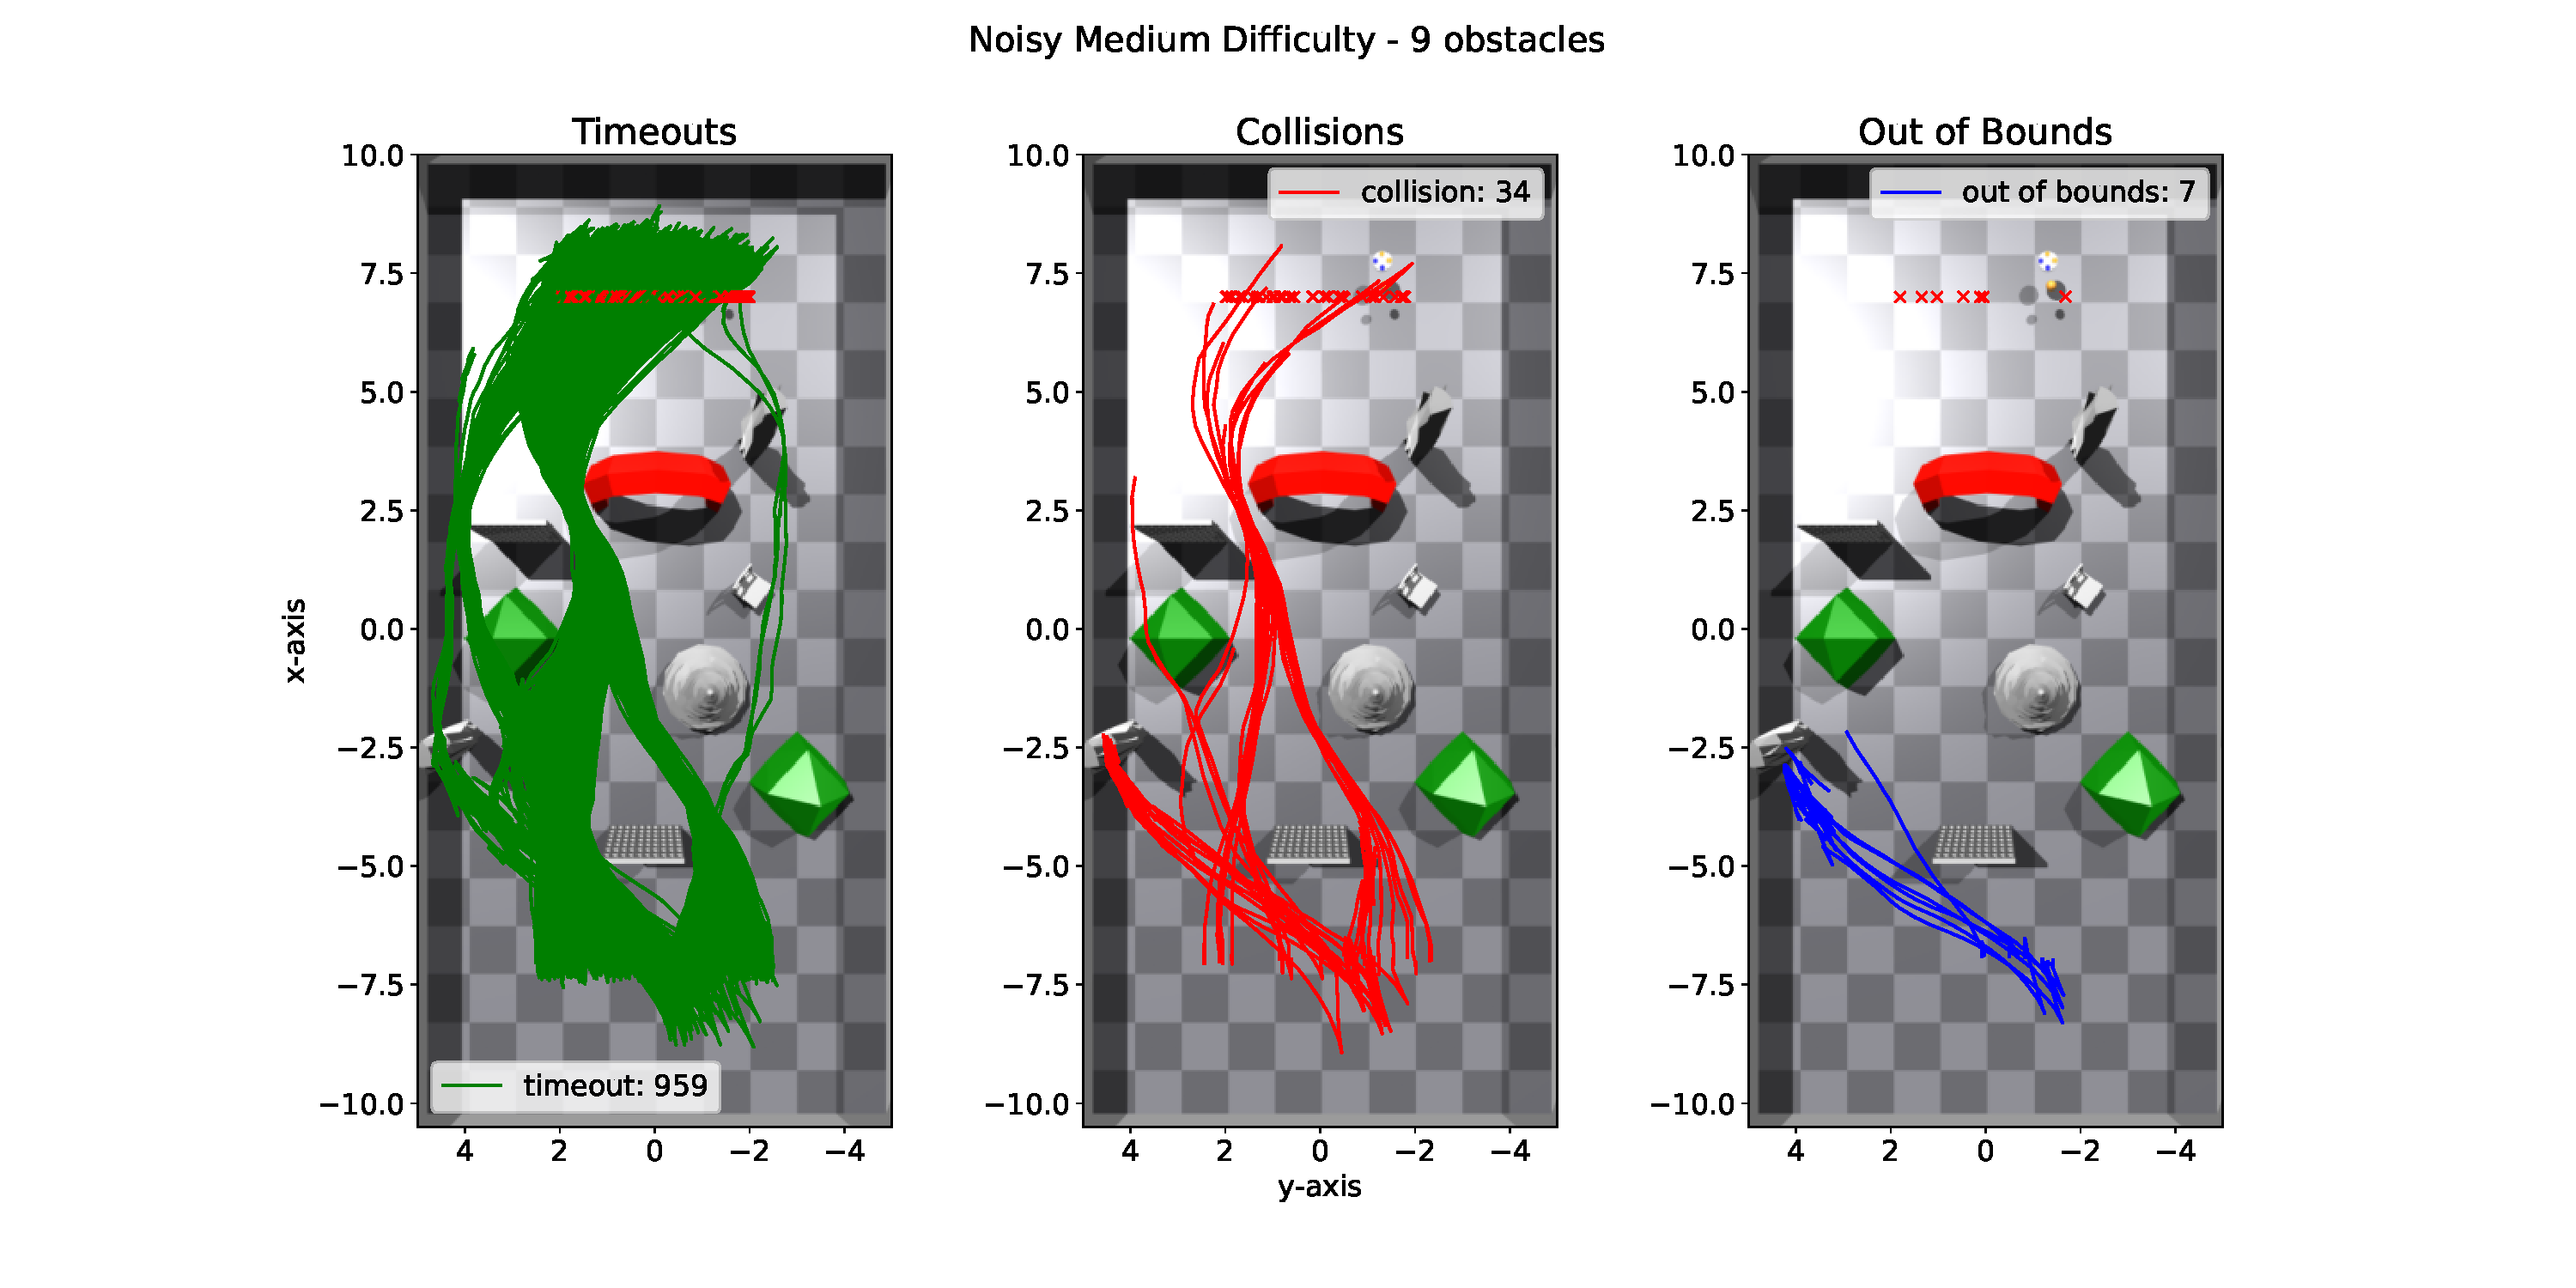
\includegraphics[width=1.2\textwidth]{figures/7_2/medium_random.pdf}
    }
    \caption{Noisy medium environment, with a timeout rate of 95.9\%. The policy is still capable of entering tight spaces when approaching them directly.}
    \label{fig:7_medium_random}
    \centering
    \makebox[\textwidth]{
    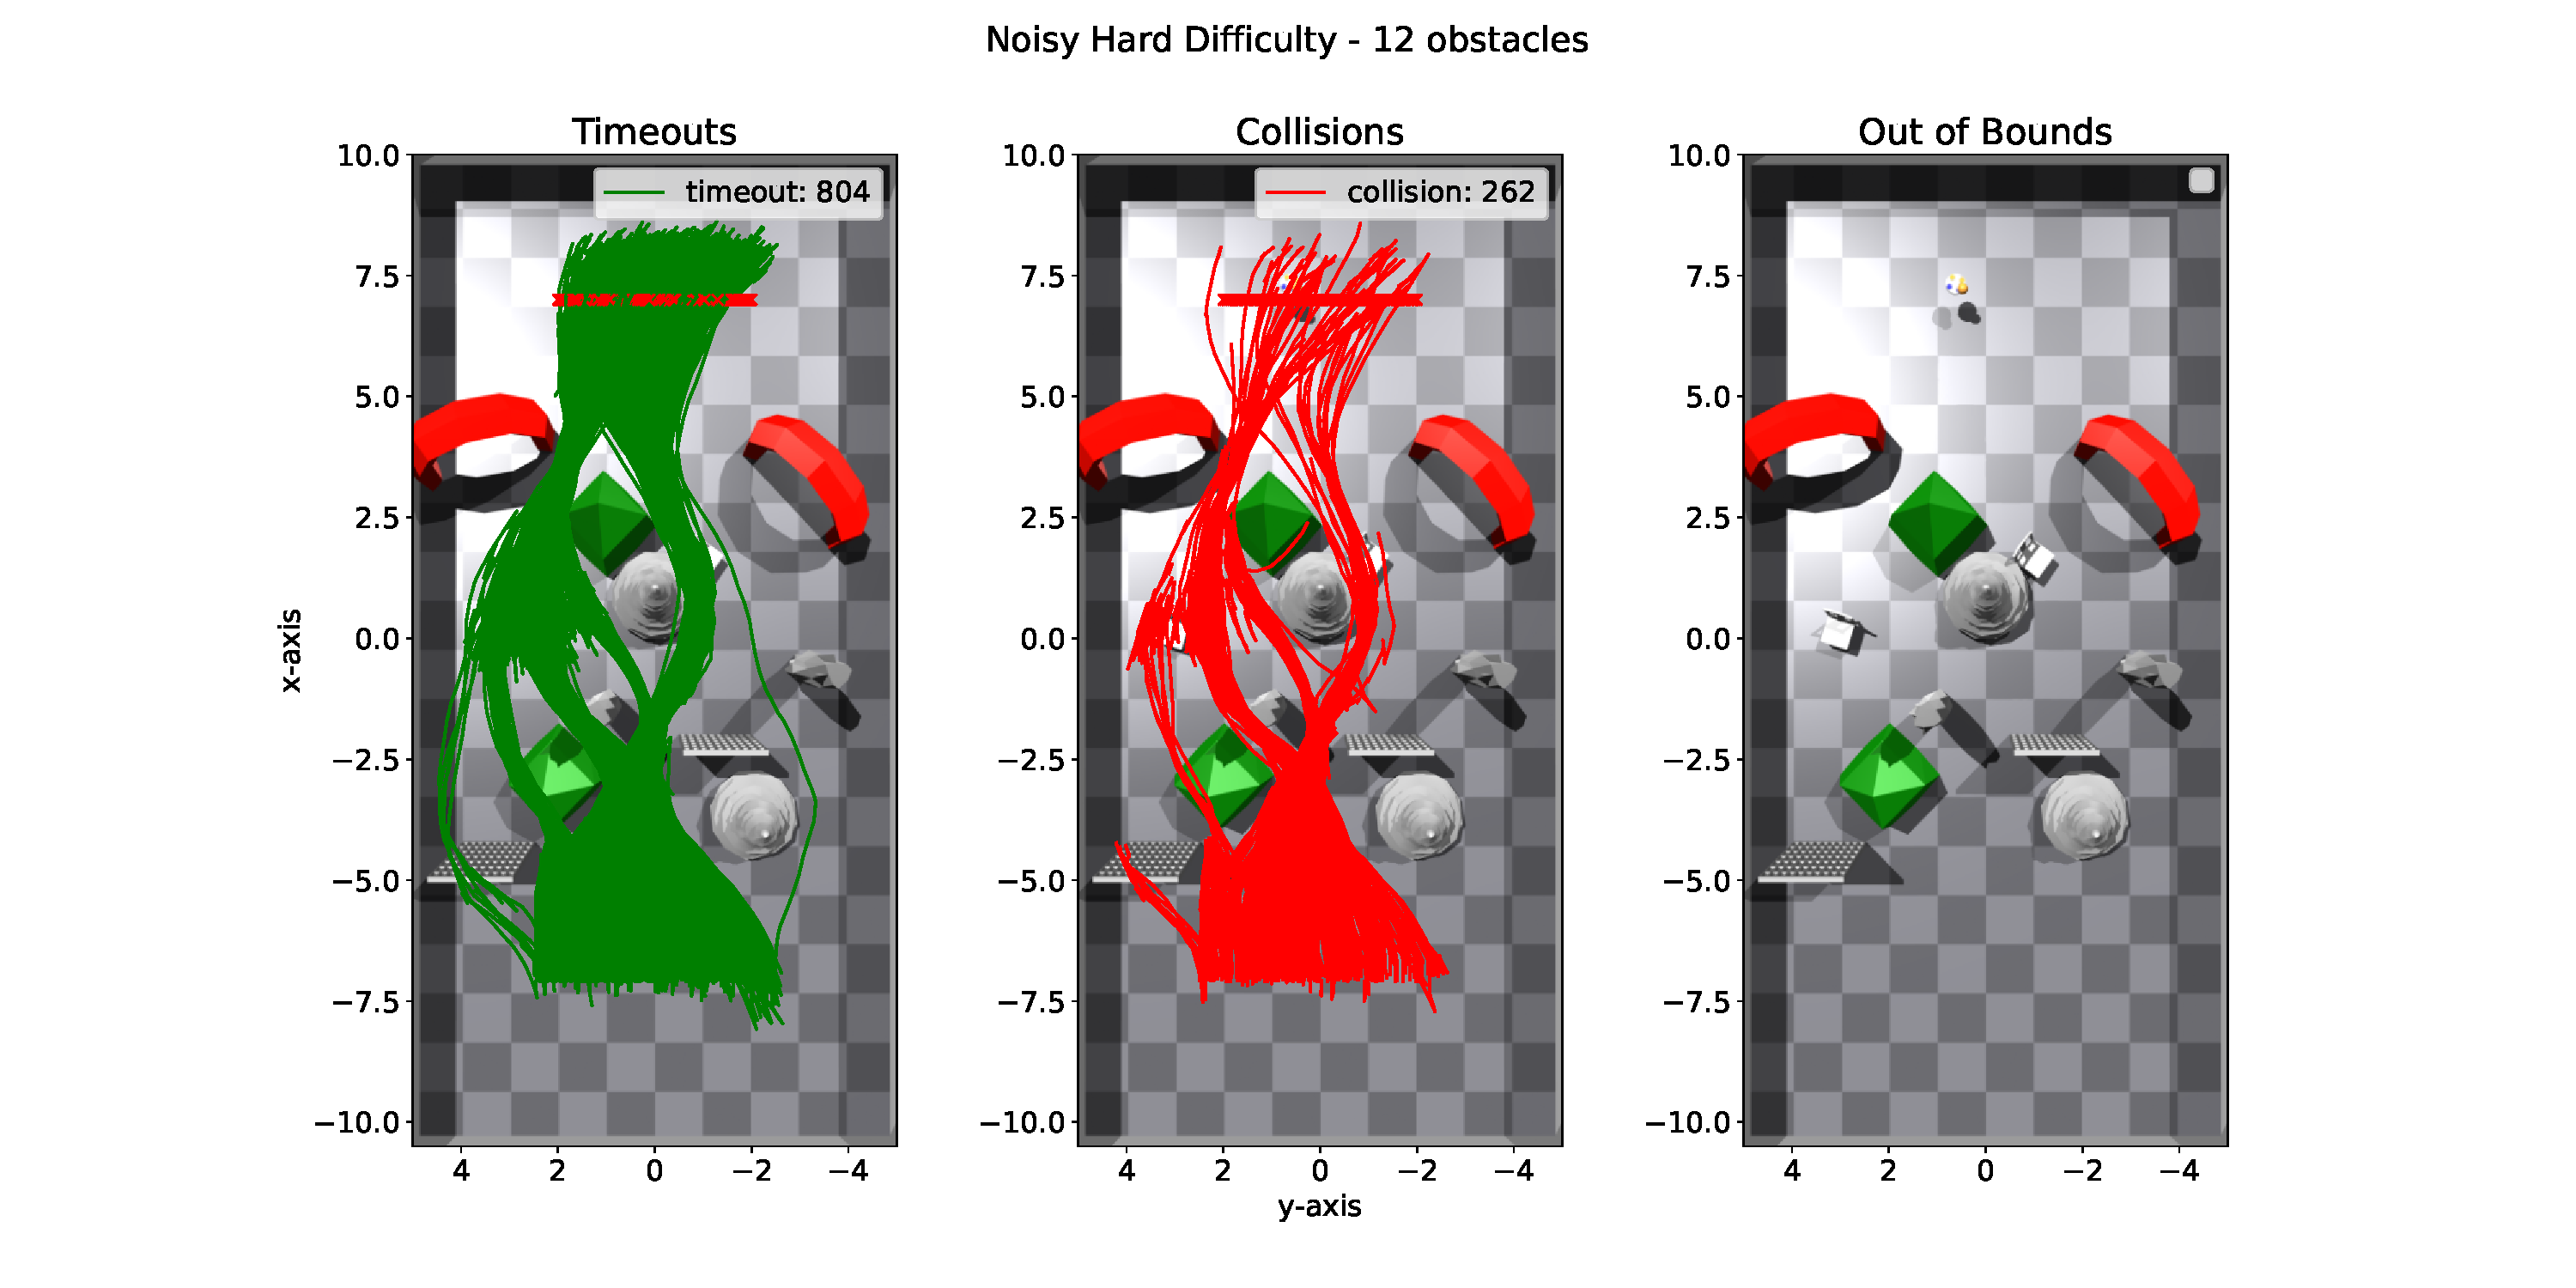
\includegraphics[width=1.2\textwidth]{figures/7_2/hard_random.pdf}
    }
    \caption{Noisy hard environment, with a timeout rate of 75.4\%. The effects of noise are more prevalent when careful navigation is required. A larger distribution of trajectories is observed along with much more reversing.}
    \label{fig:7_hard_random}
\end{figure}
\begin{figure}[htb]
    \centering
    \makebox[\textwidth]{
    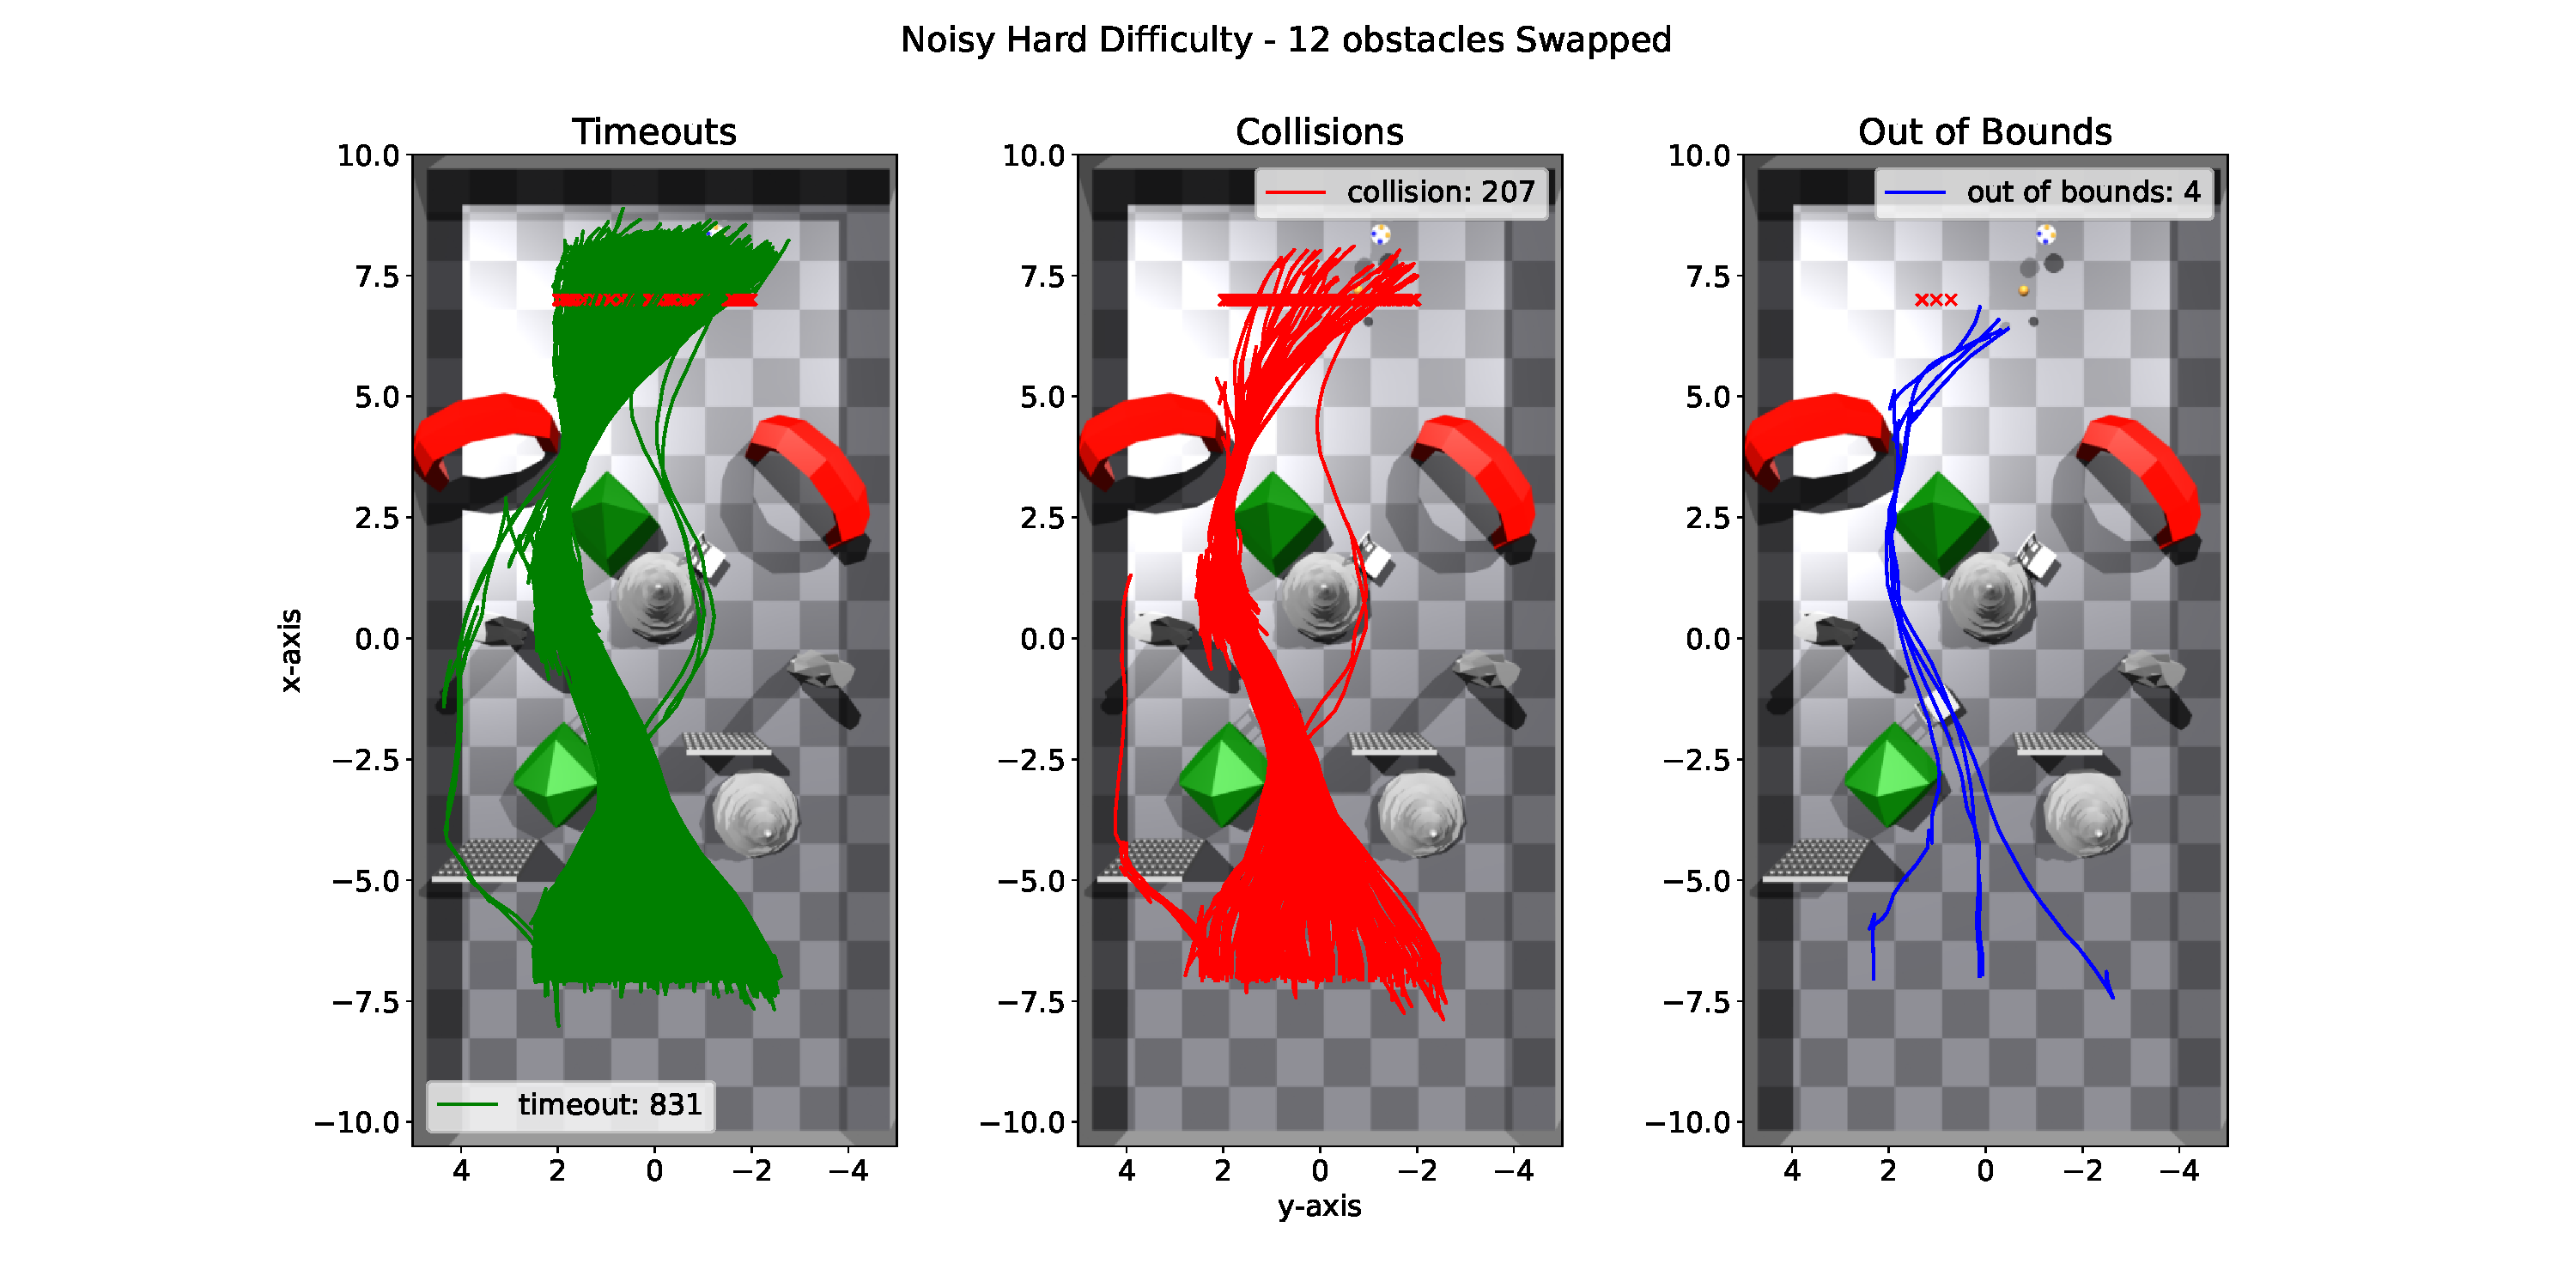
\includegraphics[width=1.2\textwidth]{figures/7_2/hard_swapped_random.pdf}
    }
    \caption{Noisy hard environment with swapped simple stone and chair, and a timeout rate of 79.8\%. The policy performance in very tight spaces is significantly impacted due to small variations in observed state and actions. As a result, many more collisions occur in along the formerly optimal path.}
    \label{fig:7_hard_swapped_random}
\end{figure}

Surprisingly, the agent does very well to adapt to noise, having more-or-less the same collision statistics. We note that the main difference is in the hard-swapped environment, where the number of collisions have increased from 14 to 207. Otherwise, we also see a slight increase in the number of out-of-bounds events. To get a better understanding, we can examine Figures \ref{fig:7_easy_random}, \ref{fig:7_medium_random}, \ref{fig:7_hard_random} and \ref{fig:7_hard_swapped_random}.

The first consequence of noise is that we observe a greater distribution of trajectories taken towards goal. If we consider what states the quadrotor has, the ones which are the most significant for waypoint navigation are the position, velocity and yaw rate. Since we add noise to these states, we can imagine that the quadrotor applies corrective behaviour to its action in response to changes in its state, which explains a more raggedness in the trajectories of the quadrotor. However, the a possible risk is the combination of corrective actions along with noise in the action -- which could lead to imperfect manoeuvring and thus collision.  

From the easy environment in \cref{fig:7_easy_random}, we note that the increased risk of collision is almost non-existent, as the collision rates have actually dropped in comparison to before. This affirms the quadrotor conservative behaviour where it does not necessarily take risky behaviours and maintains a reasonable distance from obstacles. However, in more cluttered environments, we see that the quadrotor is more susceptible to collisions simply because it is forced to take narrow routes. This is also apparent in \cref{fig:7_hard_swapped_random}, where previously it could navigate fine through the opening at the end, though suffers the bulk of its collision there in the noisy case.

Another feature of noise is that we see a greater display of reversing, particularly in the hard environment by comparing \cref{fig:7_hard} and \cref{fig:7_hard_random}. This suggests that the quadrotor has learned not only to reverse when it the path ahead seems blocked, but also in the case of poor quadrotor placement in regards to obstacles. Rather than risking a collision, it was observed that the agent would simply oscillate back and forth as an attempt to reorient itself or find new paths. This also illustrates why a conservative policy would gather less rewards, while managing to maintain low collision rates.

Despite the reasonable noise in the agent states and actions -- a $>60\%$ chance of more than a $10\%$ noise factor -- the quadrotor still outperforms our expectations, where see that it is only in the very tight spaces where we observe the adverse effects of noise. As mentioned, this can be attributed to the quadrotor deciding on conservative paths to avoid being close to obstacles and it backing away if it perceives the path to be to risky. However, another justification is that PPO makes use of a stochastic policy from which actions are sampled. This means that there is already a layer of randomness in the the agent actions, which the policy has has accounted for to ensure robust performance, which therefore minimises the effects of additional noise in the action space.


\subsection{Robustness to Noise in Depth Images}
Another possible reason for why the policy adapted well to noise in the previous chapter is because the depth images were still perfect. We justified that the positions, velocities and yaw rate observations were perhaps not that important since the quadrotor has planned good paths that account for stochastic behaviour. But what happens if we add noise to the agent's main tool for motion planning? To explore this, we perform another robustness test, this time to both the depth images, and the state and actions of the agent. We also choose the noise to be \textit{additive} white Gaussian noise instead of multiplicative, with the noise parameters $\epsilon_n \sim \mathcal{N}(0, 0.05)$. Effectively, due to the ``naive'' processing of depth images in our agent, this results in many white and black speckles in the depth images received by our VAE, seen clearly in \cref{fig:7_noisy_depth_png}.

We can observe that the simulated noise is not that realistic, as compared to e.g. the ones in \cite{HighSpeedFlightWild}, as is by no means an example on how to train a quadrotor for zero-shot transfer to real environments. Yet, since the agent has never experienced any effects of noise to depth images, it serves to illustrate the consequence of suddenly experiencing it.
\begin{figure}[H]
    \centering
    \begin{subfigure}[b]{0.49\textwidth}
        \centering
        \captionsetup{justification=centering}
        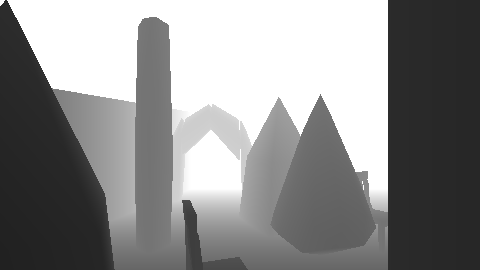
\includegraphics[width=0.98\textwidth]{figures/7_2/11_0_a_pre_image.png}
        \caption{Input depth image}
        \label{fig:11_0_a_pre_image}
    \end{subfigure} 
    \hfill
    \begin{subfigure}[b]{0.49\textwidth}
        \centering
        \captionsetup{justification=centering}
        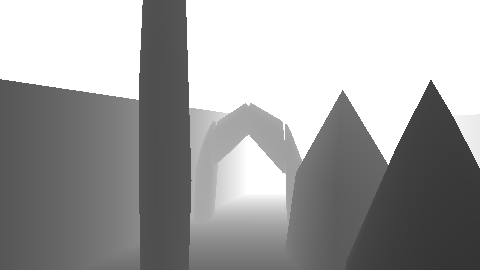
\includegraphics[width=0.98\textwidth]{figures/7_2/60_0_a_pre_image.png}
        \caption{Input depth image}
        \label{fig:60_0_a_pre_image}
    \end{subfigure}
    \\
    \begin{subfigure}[b]{0.49\textwidth}
        \centering
        \captionsetup{justification=centering}
        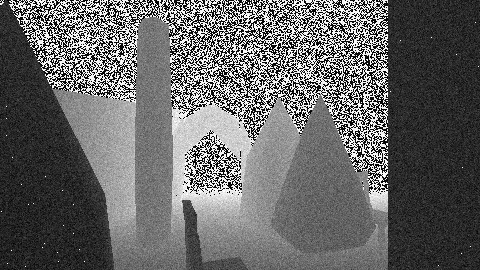
\includegraphics[width=0.98\textwidth]{figures/7_2/11_0_b_post_image.png}
        \caption{Noise added}
        \label{fig:11_0_b_post_image}
    \end{subfigure} 
    \hfill
    \begin{subfigure}[b]{0.49\textwidth}
        \centering
        \captionsetup{justification=centering}
        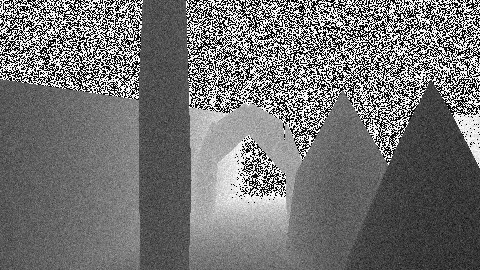
\includegraphics[width=0.98\textwidth]{figures/7_2/60_0_b_post_image.png}
        \caption{Noise added}
        \label{fig:60_0_b_post_image}
    \end{subfigure} 
    \\
    \begin{subfigure}[b]{0.49\textwidth}
        \centering
        \captionsetup{justification=centering}
        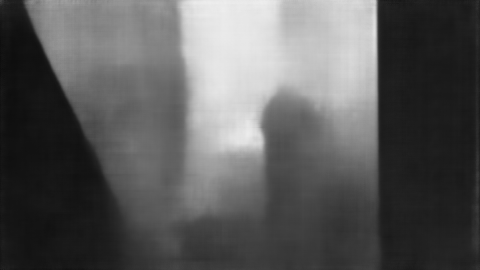
\includegraphics[width=0.98\textwidth]{figures/7_2/11_0_c_vae_image.png}
        \caption{Decent reconstructed output}
        \label{fig:11_0_c_vae_image}
    \end{subfigure} 
    \hfill
    \begin{subfigure}[b]{0.49\textwidth}
        \centering
        \captionsetup{justification=centering}
        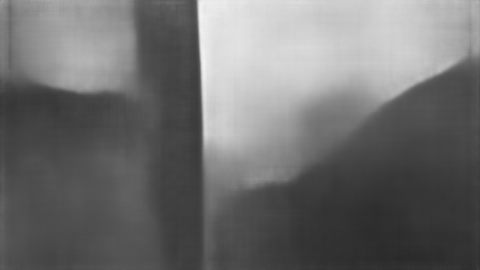
\includegraphics[width=0.98\textwidth]{figures/7_2/60_0_c_vae_image.png}
        \caption{Poor reconstructed output}
        \label{fig:60_0_c_vae_image}
    \end{subfigure}
    \caption{The effects of additive Gaussian white noise $\epsilon_n \sim \mathcal{N}(0, 0.05)$ to our depth images received by our network. Their reconstructed depth images are also shown. Recall that the VAE reconstructs a filtered version of inputs. We observe that in some cases performs decently, while other times imagining ``phantom obstacles'' that are very close.}
    \label{fig:7_noisy_depth_png}
\end{figure}

We see the adverse effect of noise in \cref{fig:hard_swapped_random_depth}, where the performance of the agent is severely impeded.
\begin{figure}[htb]
    \centering
    \makebox[\textwidth]{
    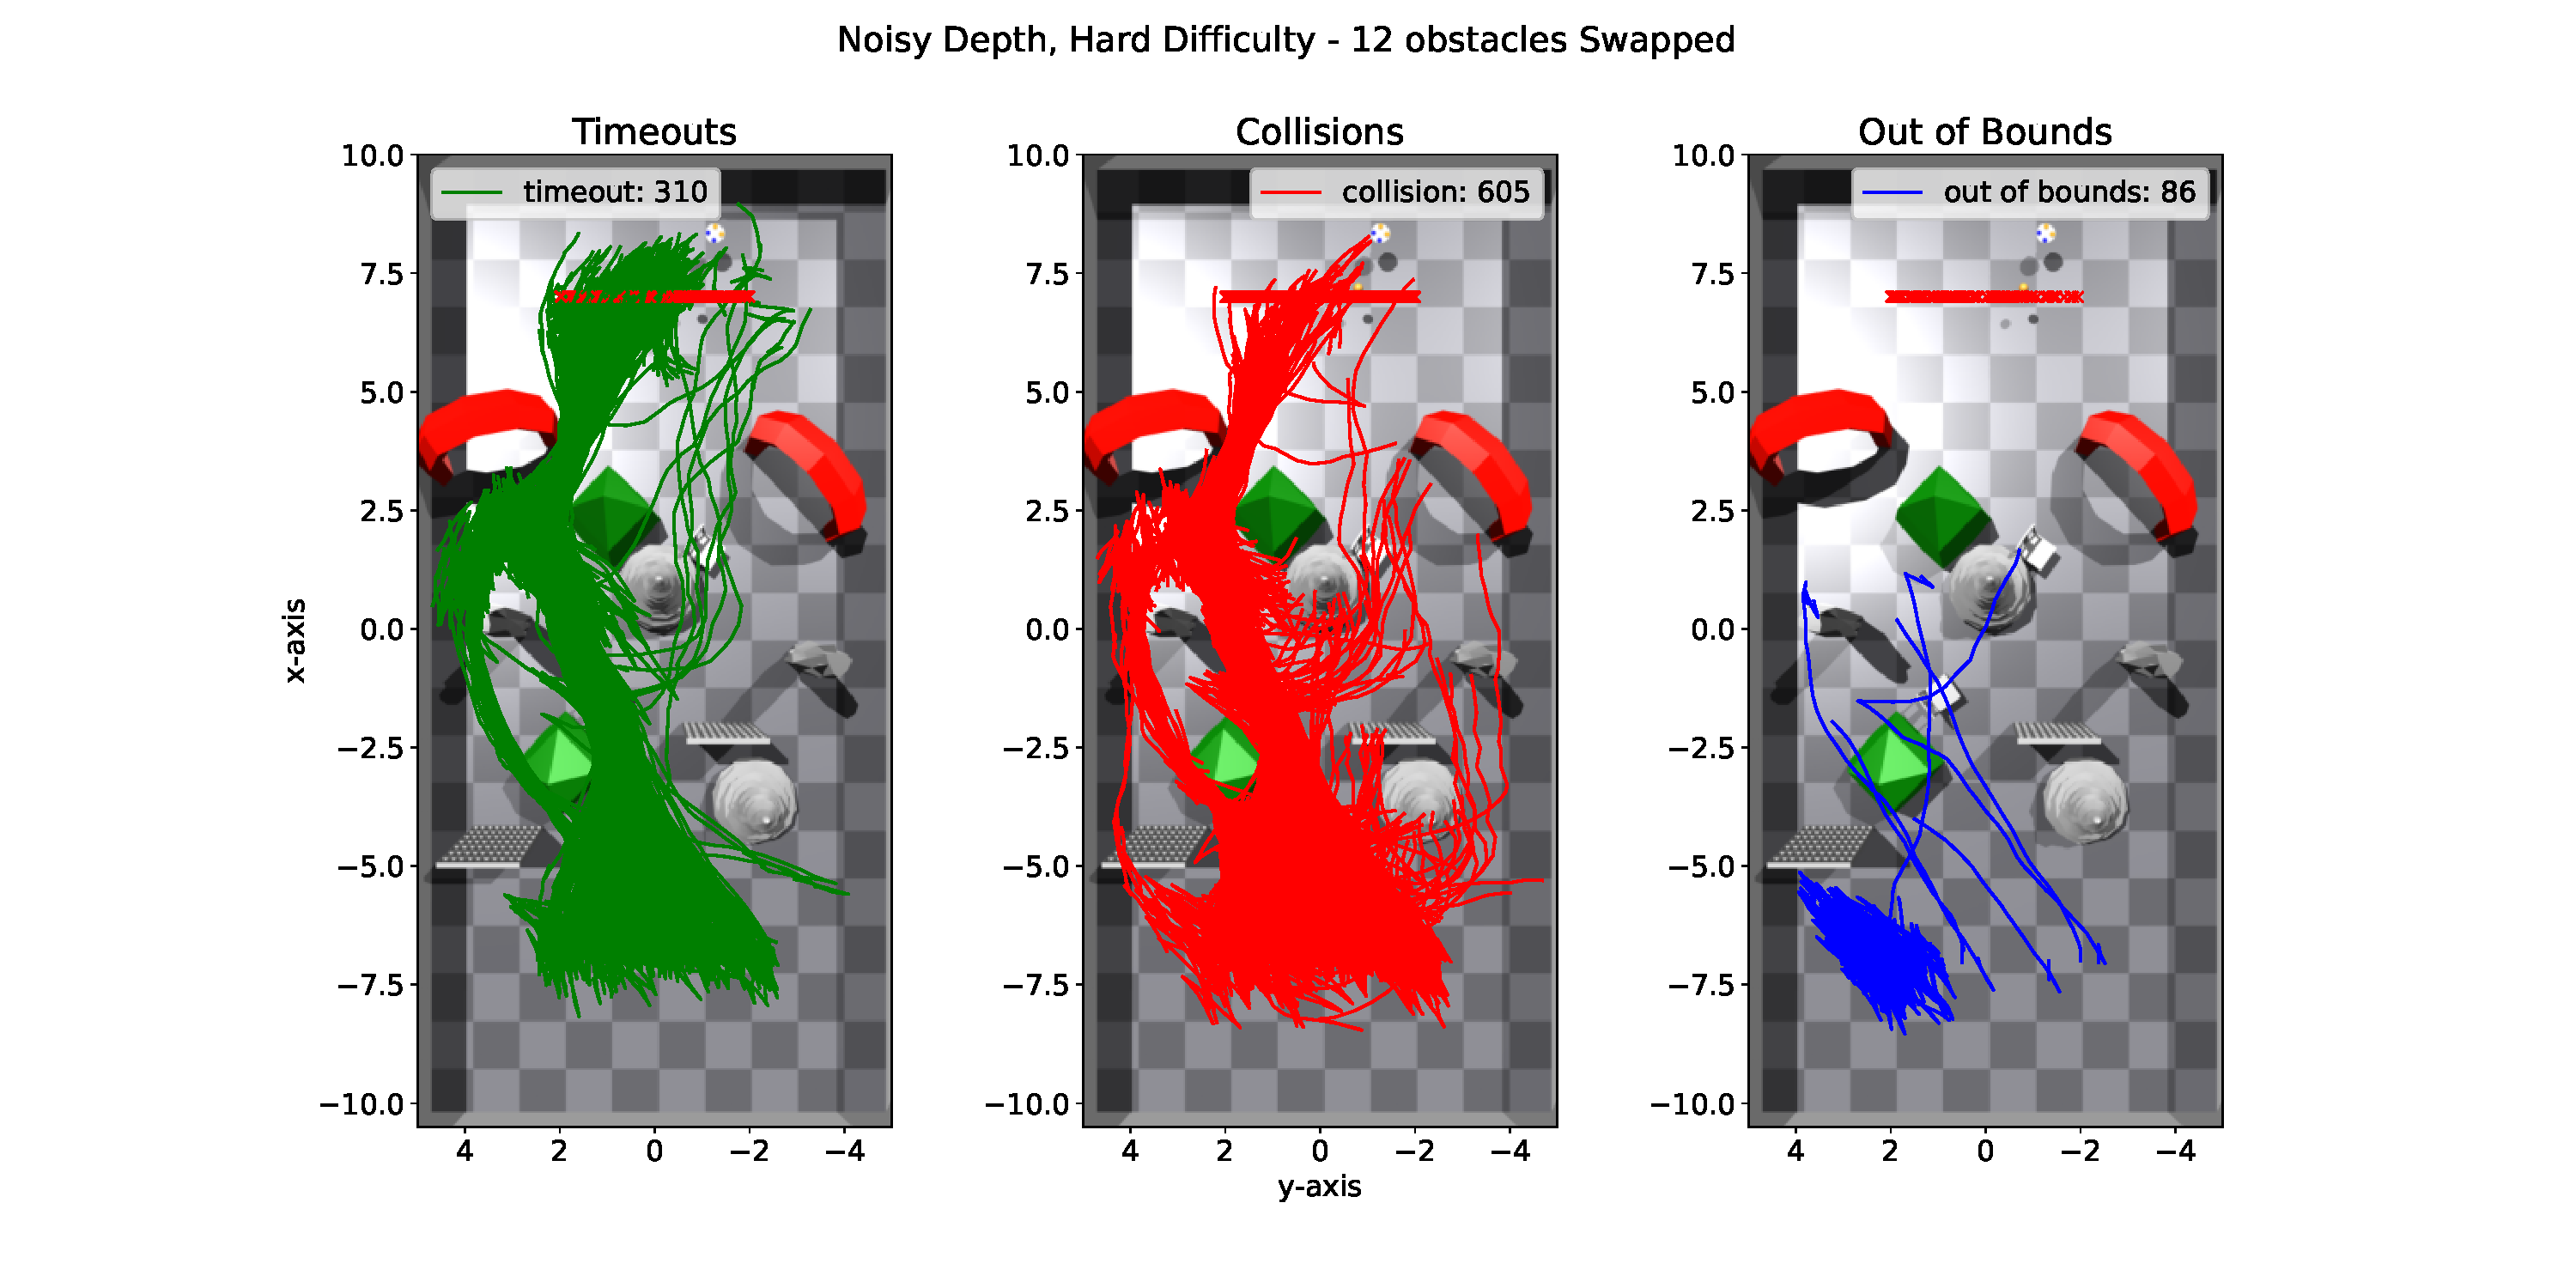
\includegraphics[width=1.2\textwidth]{figures/7_2/hard_swapped_random_depth.pdf}
    }
    \caption{The swapped hard environment with Gaussian white noise $\epsilon_n \sim \mathcal{N}(0, 0.05)$ added to depth images, agent states and actions. The timeout rate is now at $31.0\%$, dramatically reduced from previous cases.}
    \label{fig:hard_swapped_random_depth}
\end{figure}
First, we can note a very varied trajectory distribution and substantial amount of collisions. We see that this test demonstrates the importance of accurate depth images for motion planning whereby the agent struggles to map the noisy depth images to proper actions. As a result, we observe excessive turning in all directions, and also a lot of reversing. 
This results in a lot of collisions as the experiences many pass-by collisions and reversing collisions.

Interestingly, a rare behaviour that was not previously observed was the policy's ability to travel backwards (opposite of $\p_t$) so to navigate past obstacles and reach goal. This can be seen in the timeout plot where the agent frequently attempted to make its away around pine tree. However, we see that in many cases this resulted in crashing directly into the top of the tree.

Overall, this performance is expected since we have never exposed either our VAE our navigation policy to noisy depth images. This leads to a propagation of error through our model, since we are unaware of the consequence this noise has in our latent space, nor the effect this noise-in-the-latent-space has on our agent actions. Nevertheless, similarly to \cite{LearningStateRepresentation}, this can be mitigated by training the VAE to also learn how to filter real or noisy depth images, such that it performs both dilation and denoising. Otherwise, we can also simulate noise our simulation depth images and train a policy which receives these noisy depth images as input, such that it learns to account for this in some degree, like in \cite{HighSpeedFlightWild}.



\subsection{Larger Environments}
For our final evaluation study, we attempt to run the policy in larger environments. This should demonstrate the generalisation capability of the policy when introduced to a new state space distribution. Particularly, we have observed that the agent is capable in decently sized environments, adept at navigating through 8m of obstacles. In this case, we set the environment size to be $30\times15$, such that the effective obstacle area is $18\cdot15 = 270$, and set the number of obstacles to be 25. 
With this, we obtain the results in \cref{fig:7_large_env_9_policy}.
\begin{figure}[htb]
    \centering
    \makebox[\textwidth]{
    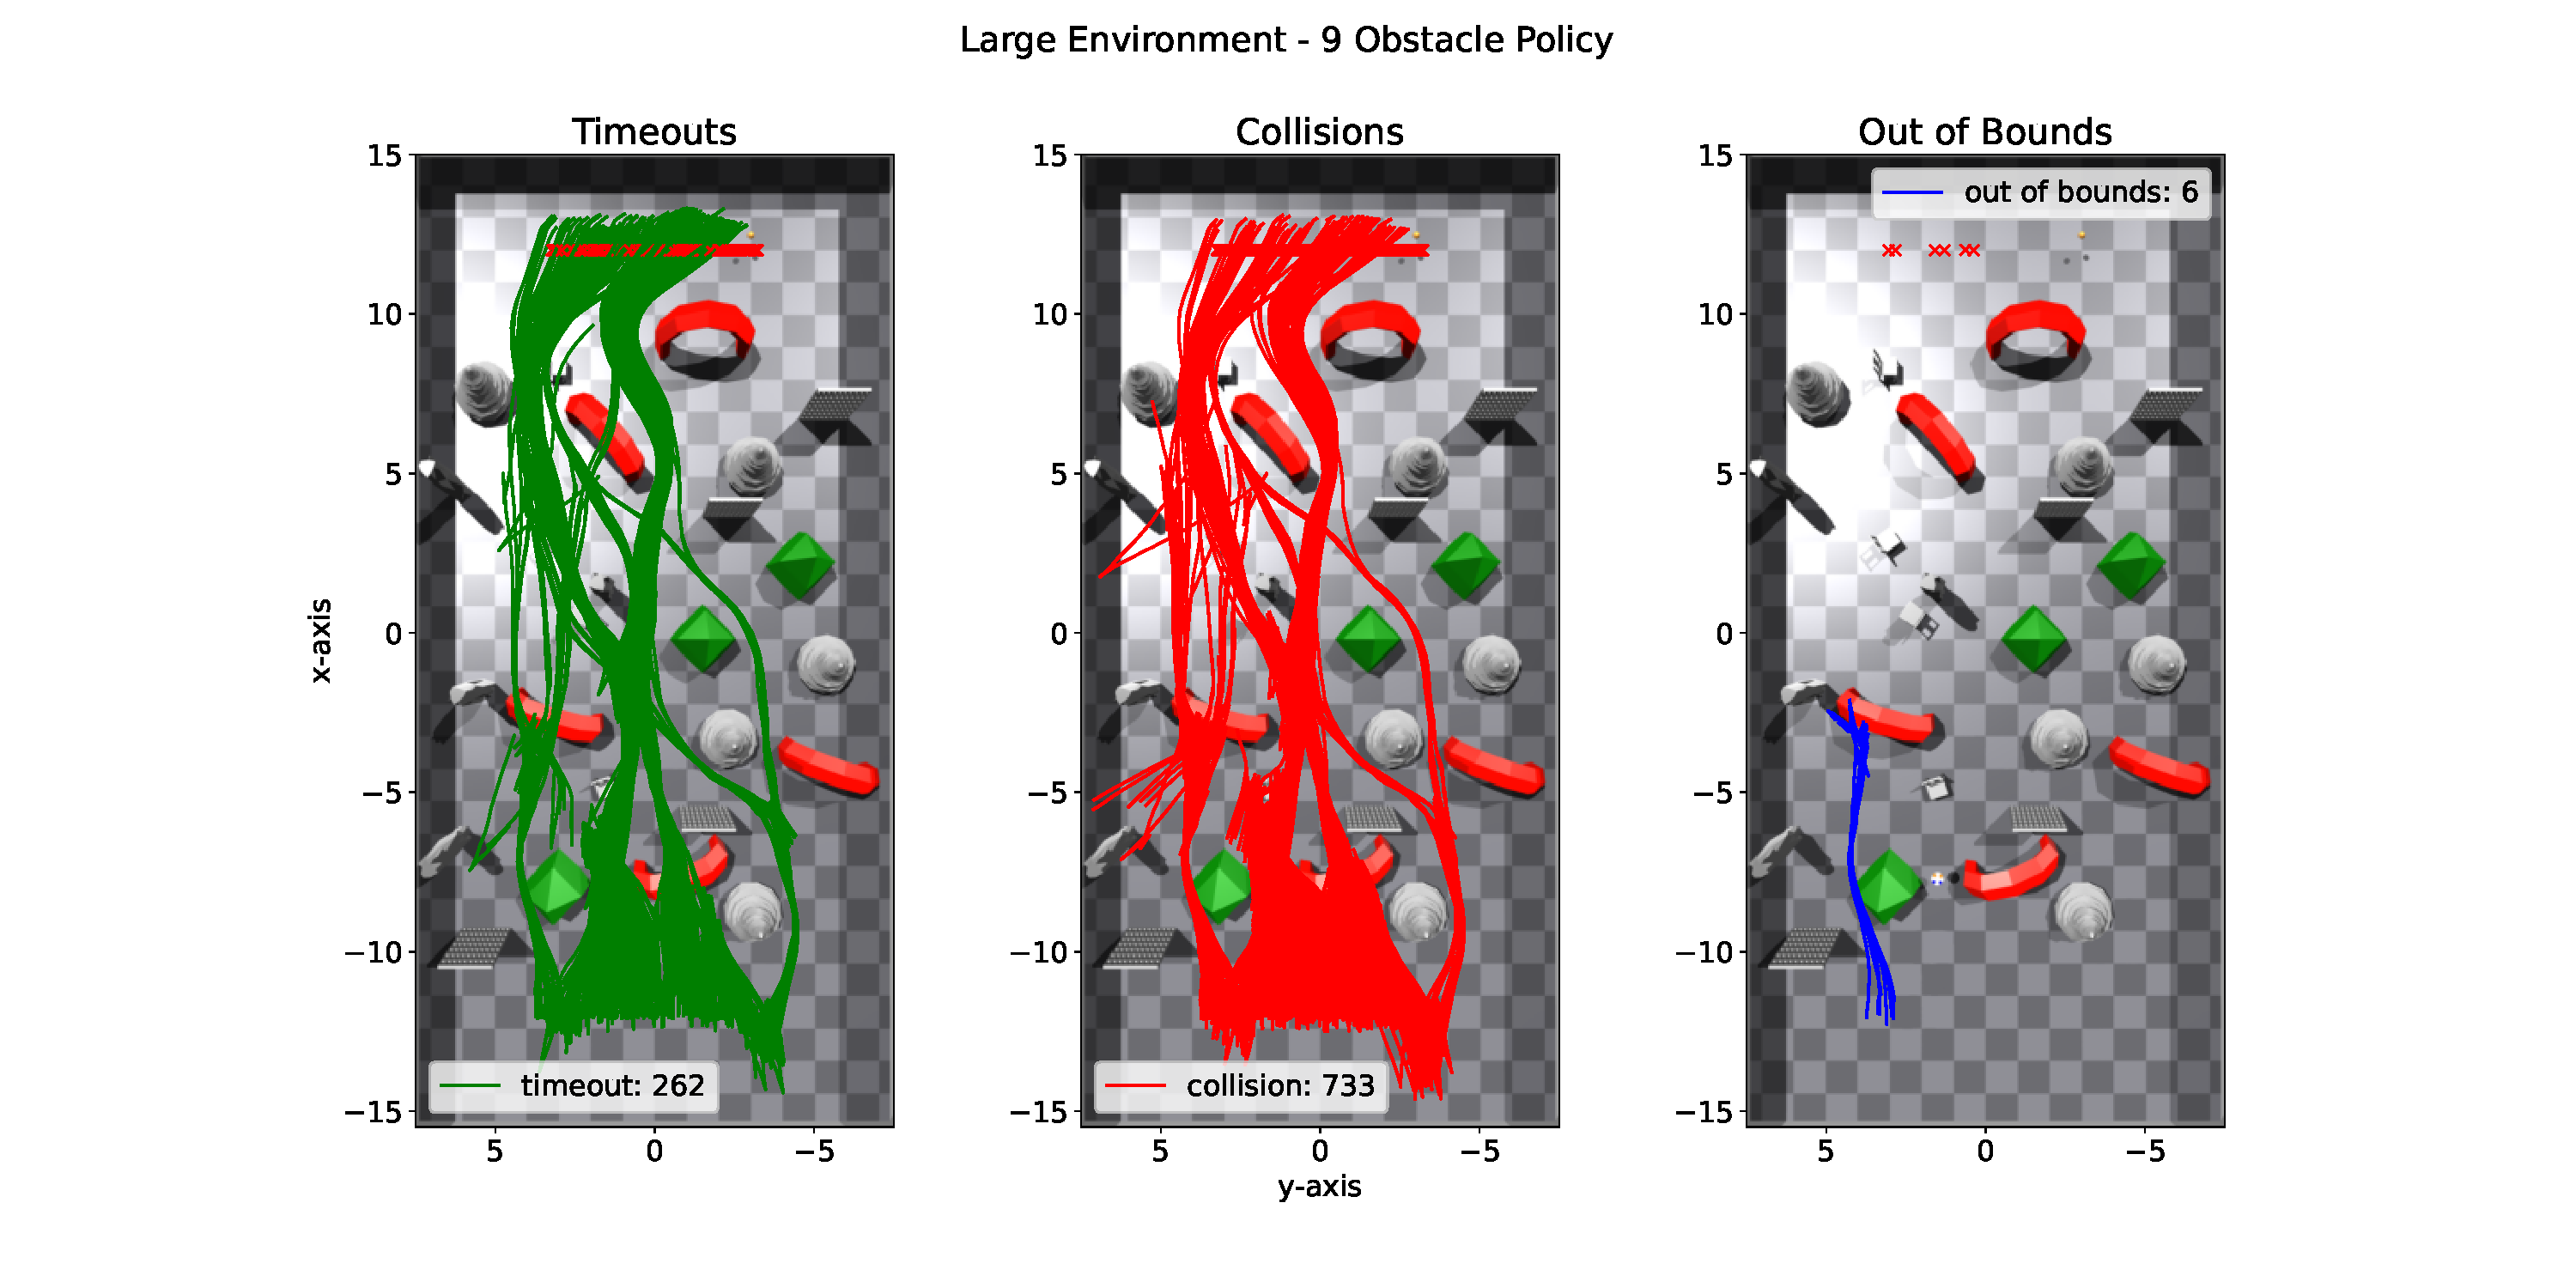
\includegraphics[width=1.2\textwidth]{figures/7_2/large_env_9_policy.pdf}
    }
    \captionsetup{justification=centering}
    \caption{The large environment with 25 obstacles in an area $[30, 15]$ area. The timeout rate is 26.2\%.}
    \label{fig:7_large_env_9_policy}
\end{figure}

Based on the results, we see that the policy has performs poorly, colliding with obstacles 73.3\% of the time. There could be several reasons for this, the first of which is a poor generalisation to larger environments, for example through seeing obstacles relatively early and much later. This means that because there is a lack of experience in these states-obstacle combinations, we cannot expect that the policy provides as finely-tuned actions as in the normal cases. We also can observe that the trajectories taken by the agent are mostly confined in $y \in [-5, 5]$. This further suggests that our agent has learnt to exploit the small environment -- essentially ``over-fitting'' it -- which comes at the cost of lack of generalisation.

A more straightforward reason could be that we overestimated the policy ability to navigate past obstacles, such that when tasked to avoid roughly seven obstacles per trajectory more mistakes occur along the way. Though not so easily visible, we should also note that many of the collisions were early on as a result of trying to fly over the simple-u but not having the height to manage it. This could be due to the low spawn point of the quadrotor at roughly $1$m while needing to ascent to about 3m to pass above the simple-u. An alternative to passing the simple-u is to reverse and descend, such that it can go under the it. However, since the quadrotor is so low during the start, this also resulted in many crashes. This behaviour can also be seen by the simple-u on the left, where we see many back-and-forth motions as the quadrotor descends, unfortunately into the chair. 

Nevertheless, we expected the policy to much better than observed here, since it had essentially no problems before -- apart from too tight spaces, though this not the case here. So, to demonstrate the potential of this approach, we added two more levels to the curriculum, this time in environments of size $[24, 12]$ and later $[30, 15]$, as shown in \cref{fig:7_train_nav_25_obst}.
By testing the new policy in the same environment, we obtained the result in \cref{fig:7_large_env_new_policy}.
\begin{figure}[htb]
    \centering
    \makebox[\textwidth]{
    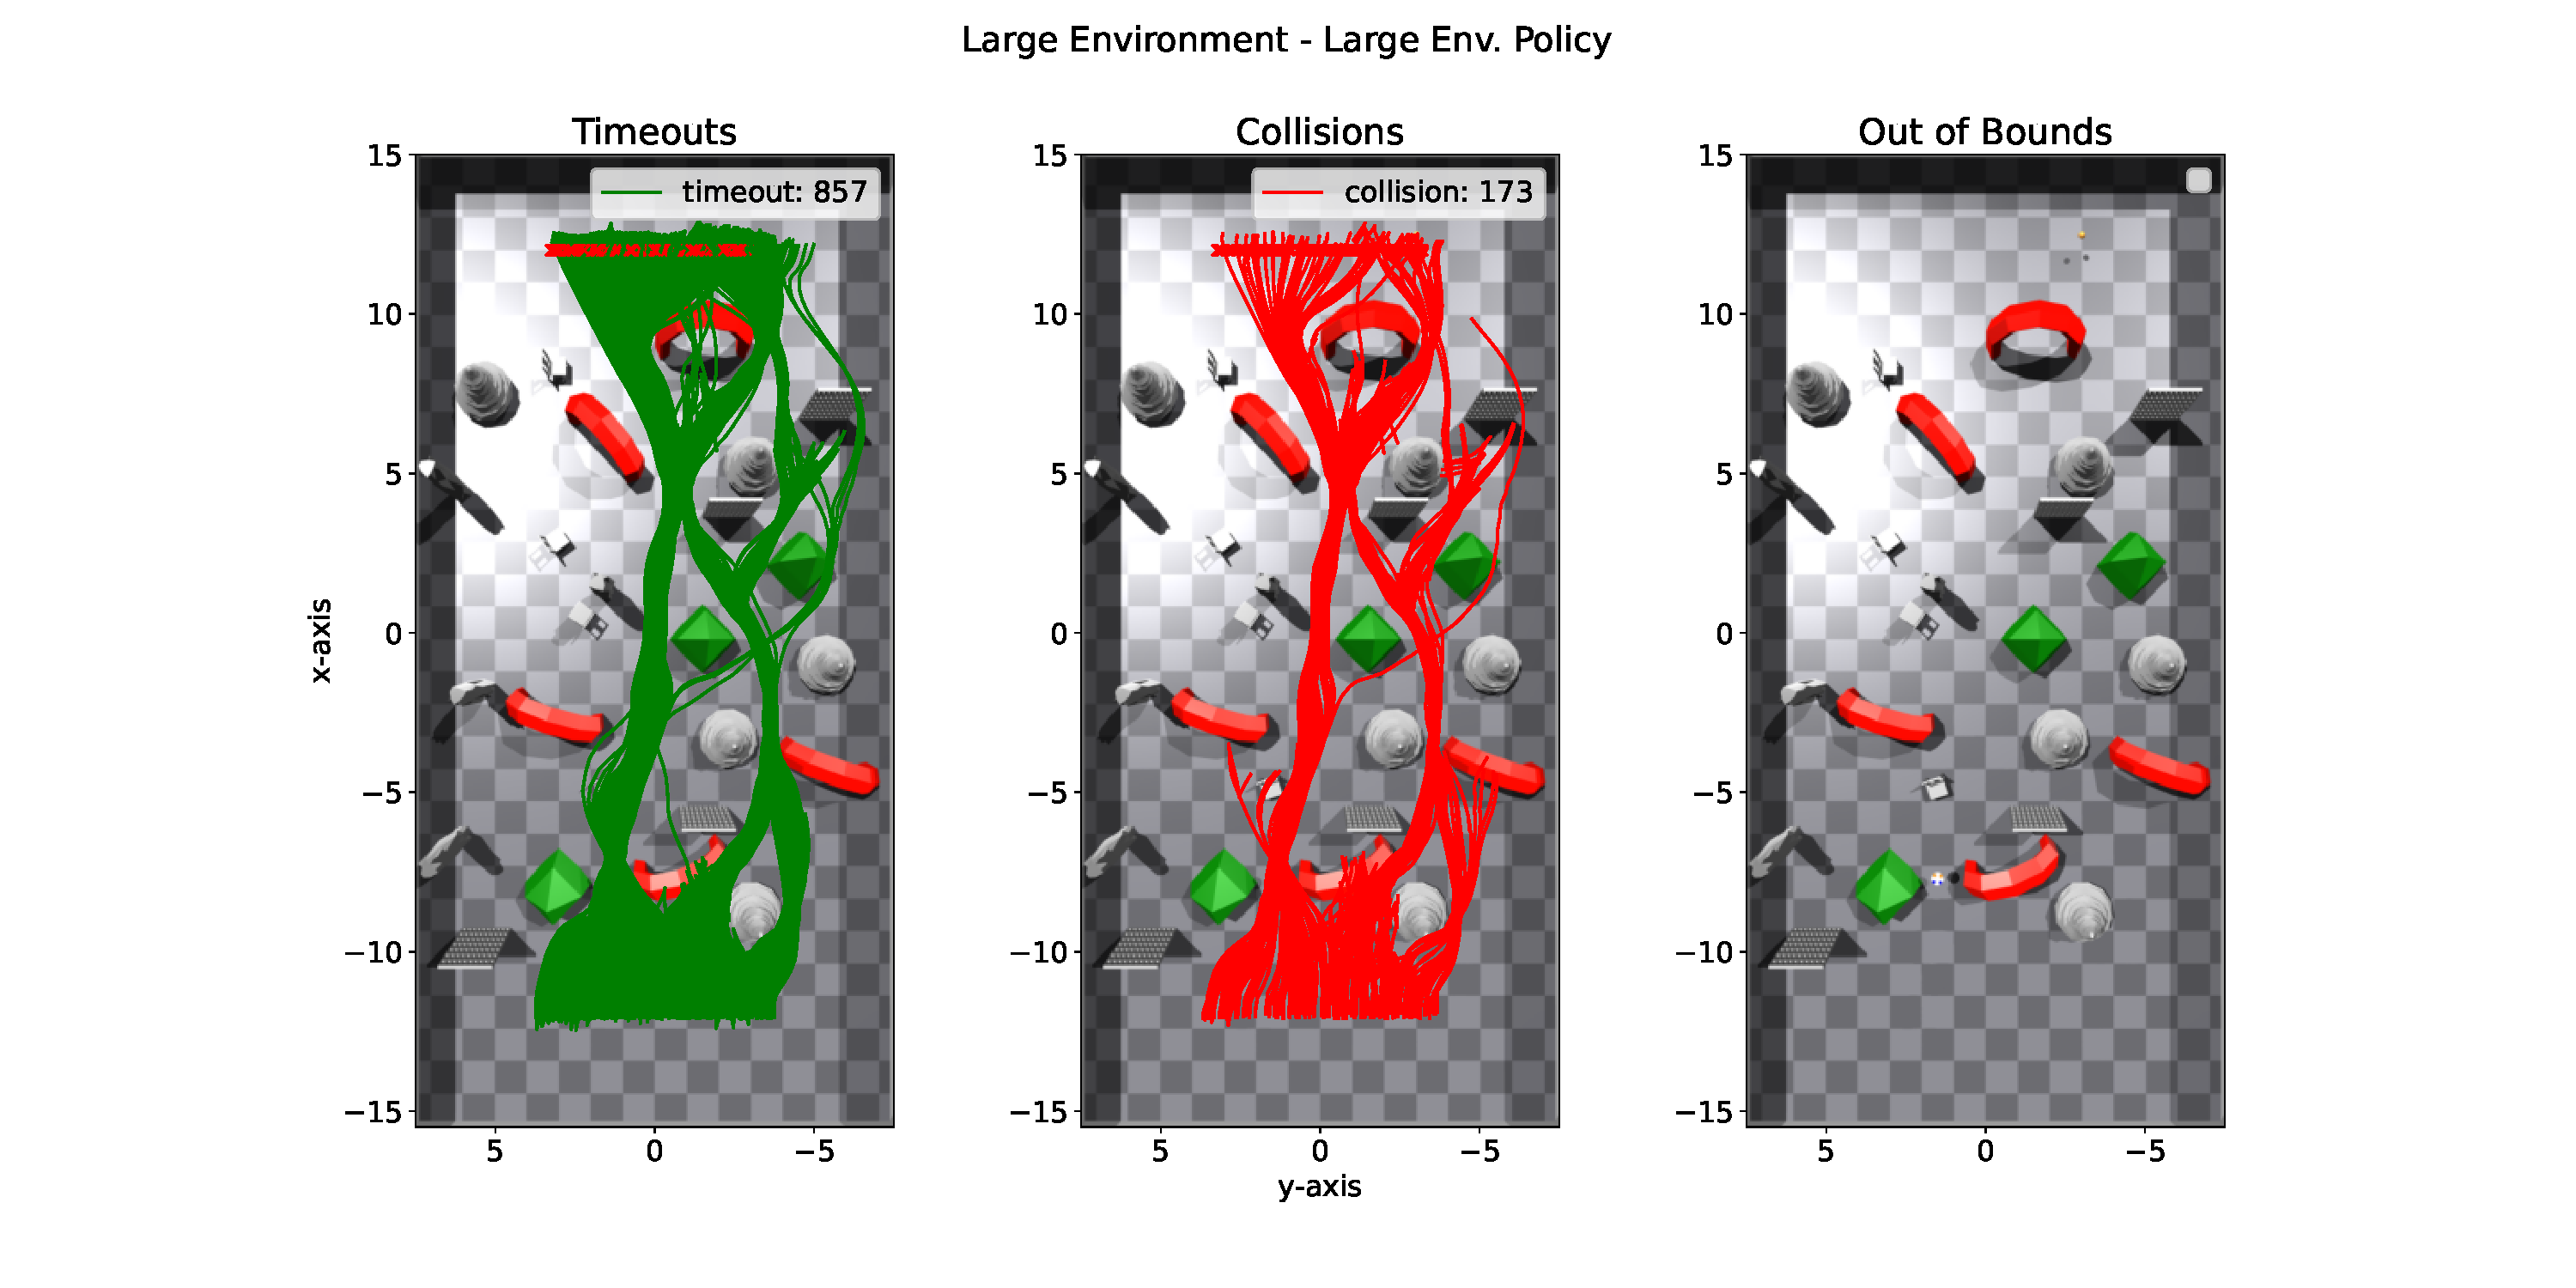
\includegraphics[width=1.2\textwidth]{figures/7_2/large_env_new_policy.pdf}
    }
    \label{fig:7_large_env_new_policy}
    \captionsetup{justification=centering}
    \caption{The new policy in a large environment, with timeout rate of 85.7\%. Training it required 7500 extra iterations compared to the 9-obstacle policy.}
\end{figure}

Here, we observe a large progression in policy performance, where the agent attains a timeout rate of $85.7\%$. Despite not matching the statistics from the earlier tests, we reason that due to the increased number additional turns per trajectory this is acceptable. From the figure, we note that collisions are still caused by similar factors which we have discussed before -- namely attempting to fly over or under simple-u's, reversing into obstacles and corner situations such as on the right at $[5, -6]$. Otherwise, another similar behaviour that it has is a favourite side, though this time predisposed to making right turns.
